\documentclass[a4paper]{article}

\usepackage[utf8]{inputenc}
\usepackage[T1]{fontenc,url}
\usepackage{cite}
\usepackage{hyperref}
\usepackage{amsmath, amssymb}
\usepackage{tikz}
\usepackage{graphicx}
\usepackage{parskip}
\usepackage{lmodern}
\usepackage{algorithm}
\usepackage{algpseudocode}
\usepackage{epigraph}
\usepackage{listings}
\usepackage{float}
\usepackage{subcaption}

\begin{document}
\title{FYS-STK4155 -- Project 1}
\author{Jing Sun and Endrias Getachew Asgedom}

\maketitle
\begin{abstract}
\noindent
Linear regression methods including the Ordinary Least Squares (OLS), Ridge, and LASSO are used in this project for analysing a numerically generated and a real satellite image data sets. The numerical dataset uses the Franke function while the satellite image is a digital topography of the west coast of Norway. The three regression methods use a polynomial function of different orders to fit and predict the two data sets. The performance of the different models are evaluated using the Mean Squared Error (MSE) and $R^2$ score. The Bootstrap and K-fold cross-validation resampling methods are used respectively for analysing the bias-variance tradeoff and selecting the optimal model. For the noise contaminated Franke function, the Ridge regression performed the best, followed by the OLS regression method. However, the LASSO regression is found to be the best in predicting the test dataset of the terrain data. In general, predictions are more challenging when using the limited-size digital terrain dataset than the corresponding noisy Franke function dataset.



\end{abstract}
\newpage

\tableofcontents

\begin{center}
    GitHub repository at \url{https://github.com/endrias34/FYS-STK4155/tree/master/Project-1}
\end{center}

\newpage

%%% MACROS
\newcommand{\half}{\frac{1}{2}}
\newcommand{\dx}{{\Delta x}}
\newcommand{\bigO}{{\mathcal{O}}}


\section{Introduction}
In supervised learning, a set of training pairs consisting of input and output is given. Then, a supervised learning-based method automatically learns a certain pattern/operation from these data and maps the input to the output. Once this mapping is learned, it can then be applied to "unseen" input data and provide a prediction according to these "learned" patterns. Due to their simplicity, linear regression methods are often used as the starting point before introducing the more advanced machine learning concepts. In the context of regression, models refer to mathematical equations that describe the relationship between the independent variables (inputs) and the dependent variables (outputs). The quality of a regression model is measured based on how well its predictions match against the actual values of the "unseen" data. To evaluate a model quantitatively, error metrics have been introduced to provide a concise and useful information about the regression model. 

In this project, the OLS, Ridge and LASSO regression methods, along with cross-validation and Bootstrap resampling methods have been investigated. For the analysis we use a numerical dataset generated using the Franke function and  a digital terrain data from Norway. To test the generalizing ability of our regression model, we added noise on the numerically generated dataset. The performance of the different models are evaluated by MSE and $R^2$ score. To analyze the bias-variance tradeoff for our model, Bootstrap is introduced and we compute the MSE, bias, and variance for the different models with different orders of polynomial. For the OLS regression, the optimal order of polynomial is determined using a $5$-fold cross-validation technique. For the Ridge and LASSO regression, the optimal values of the penalty parameter $\lambda$ as well as the optimal polynomial order are determined using a $5$-fold cross-validation technique. Finally, the confidence intervals for the estimator coefficients of the three regression methods are computed using the 95$\%$ confidence level. 

The paper is organized as follows. The first two sections introduce respectively the theoretical background and the methodology. Following these we show and analyze the two data sets. Finally, we provide a set of discussion and conclusion.

\section{Theory}

In this section, a brief description of the methods adopted in this project are given, starting with an introduction to the theory of linear regression methods. In the following subsections, the basic concepts of confidence intervals and the bias-variance tradeoff will be discussed.   

\subsection{Linear regression}
\label{sec_linreg}
Given a set of dependent variables $\mathbf{y}=[y_0,y_1,\dots,y_{n-1}]^T$, the aim of a regression analysis is to find a functional relationship describing how the dependent variables vary based on the independent variables $\mathbf{x}_{i} =[x_{i}^{0}, x_{i}^{1}, \dots, x_{i}^{p-1}]$, where $\mathbf{x}_{i}$ is a $p$-dimensional feature row vector with explanatory variables running from $0$ to $p-1$. Here, the index $i=0\ldots n-1$ runs over the number of examples in the training data \cite{lec}. When there is no prior knowledge on the functional relationship between the dependent and independent variables, it is common to assume a linear relationship of the form

\begin{equation}
    \mathbf{y} = \mathbf{X}\boldsymbol{\beta} + \boldsymbol{\epsilon},
    \label{linear1} 
\end{equation}

where, $\mathbf{X} \in \mathbb{R}^{n \times p}$ is the $design$ $matrix$ with its rows containing the features and the columns representing the data points as 

\begin{equation}
    \mathbf{X}= 
    \begin{bmatrix} 
    1& x_{0}^1 &x_{0}^2& \dots & \dots &x_{0}^{p-1}\\
    1& x_{1}^1 &x_{1}^2& \dots & \dots &x_{1}^{p-1}\\
    1& x_{2}^1 &x_{2}^2& \dots & \dots &x_{2}^{p-1}\\                      
    \dots& \dots &\dots& \dots & \dots &\dots\\
    1& x_{n-1}^1 &x_{n-1}^2& \dots & \dots &x_{n-1}^{p-1}\\
    \end{bmatrix} .
    \label{design1} 
\end{equation}


The $p$-dimensional column vector $\boldsymbol{\beta} = [\beta_0, \ldots,\beta_{p-1}]^{T}$ represents the regression parameters and $\boldsymbol{\epsilon}=[\epsilon_0,\epsilon_1,\dots,\epsilon_{n-1}]^{T}$ is the added noise and it is assumed to be distributed as $\boldsymbol{\epsilon} \sim \mathcal{N}(\mathbf{0}_p,\sigma_{\epsilon}^2\mathbf{I}_{nn})$.

\subsubsection{Ordinary least squares }
Ordinary least squares regression (OLS) is a statistical method of finding an estimator which minimizes the cost function defined as the square of the $\mathbf{L}_2$-norm of the difference between the exact and estimated values 

\begin{equation}
    C(\mathbf{X},\mathbf{\beta})=\left(\mathbf{y}-\mathbf{X}\mathbf{\beta}\right)^T\left(\mathbf{y}-\mathbf{X}\boldsymbol{\beta}\right)=\vert\vert\mathbf{y}-\mathbf{X}\boldsymbol{\beta}\vert\vert_2^2.
    \label{cost_OSL}
\end{equation}


For the OLS, the regression parameters $\boldsymbol{\beta}$ can be found by minimizing the cost function


\begin{equation}
    \hat{\boldsymbol{\beta}}_{\text{OLS}}=
    \underset{\boldsymbol{\beta}\in\mathbb{R}^p}{\operatorname{argmin}} ||\mathbf{y}-\textbf{X}\boldsymbol{\beta}||_2^2 = \underset{\boldsymbol{\beta}\in\mathbb{R}^p}{\operatorname{argmin}} \,(\mathbf{y}-\mathbf{X}\boldsymbol{\beta})^T(\mathbf{y}-\mathbf{X}\boldsymbol{\beta}),
    \label{olsmin}
\end{equation}


or equivalently, in component form,

\begin{equation}
    \hat{\boldsymbol{\beta}}_{\text{OLS}}=\underset{\boldsymbol{\beta}\in\mathbb{R}^p}{\operatorname{argmin}}   \sum_{i=0}^{n-1} (y_i -{\beta}\cdot\mathbf{x}_{i})^2.
\end{equation}


If the rank$(\mathbf{X})=p$, namely, the feature predictors (columns of the design matrix) are linearly independent, then by taking the derivative with respect to $\boldsymbol{\beta}$ there exists unique solution to equation \ref{olsmin} and it is given as


\begin{equation}
    \hat{\boldsymbol{\beta}}_{\text{OLS}}= (\mathbf{X}^T\mathbf{X})^{-1}\mathbf{X}^T \textbf{y}.
    \label{eqn_ols}
\end{equation}

The OLS regression can be equivalently described as a Maximum Likelihood (ML) estimator \cite{regression}. Therefore, the variance of the ML estimator of $\hat{\boldsymbol{\beta}}_{\text{OLS}}$ is

\begin{equation}
    \text{Var}[\hat{\boldsymbol{\beta}}_{\text{OLS}}] = (\mathbf{X}^T\mathbf{X})^{-1}{\sigma}^2,
    \label{eqn_ols_var}
\end{equation}

where, the variance of the data $\sigma^2$ is often unknown, but it can be estimated by \cite{hastie}


\begin{equation}
    \hat{\sigma}^2  = \frac{1}{n-p-1}\sum_{i=0}^{n-1}(y_i-\hat{y}_i)^2,
\end{equation}

where $\hat{y} = \mathbf{X}\hat{\boldsymbol{\beta}}_{\text{OLS}}$. As shown in equation \ref{eqn_ols_var}, we need to find the inverse of the matrix $\mathbf{X}^T\mathbf{X}$ to obtain the regression parameters $\boldsymbol{\beta}$. In this process, we may meet the problem of a singular (when the determinant is $0$) or close to singular matrix. A singular matrix does not have a matrix inverse, and trying to calculate the inverse of a near singular matrix directly is numerically unstable. This is especially a problem when the number of data points is close to or even less than the number of features. To avoid this problem, the matrix inverse may be solved using the Singular Value Decomposition (SVD), which can decompose any general matrix $\mathbf{X}$ into terms of a diagonal matrix and two orthogonal/unitary matrices \cite{lec}.

In the following sections, two regularization methods will be introduced to restrict the features and solve the problem of overfitting. The first one uses the L2-norm penalty and it is named Ridge regression. The second one has an L1-norm penalty and it is known as LASSO regression.

\subsubsection{Ridge regression}

Both Ridge and LASSO regressions can be regarded as modifications to OLS, where the cost function now has an extra term, the regularization penalty. In Ridge-regression, the penalty $E_{Ridge}$ is taken to be the $\mathbf{L}_2$-norm of the regression parameters $\boldsymbol{\beta}$


\begin{equation}
    E_{Ridge}= \lambda ||\boldsymbol{\beta}||_2^2 = \lambda \boldsymbol{\beta}^T \boldsymbol{\beta},
\end{equation}


where the constant $\lambda$ is a tuning parameter and it controls how much the penalty weighs. The cost function for Ridge regression can be then written as


\begin{equation}
    C(\mathbf{X},\boldsymbol{\beta};\lambda)=(\mathbf{y}-\mathbf{X}\boldsymbol{\beta})^T(\mathbf{y}-\mathbf{X}\boldsymbol{\beta})+\lambda\boldsymbol{\beta}^T\boldsymbol{\beta},
    \label{cost-ridge}
\end{equation}


or


\begin{equation}
    C(\mathbf{X},\boldsymbol{\beta};\lambda)=
    \vert\vert\mathbf{y}-\mathbf{X}\boldsymbol{\beta}\vert\vert_2^2+\lambda ||\boldsymbol{\beta}||_2^2.
\end{equation}

The Ridge regression estimation of the regression parameters $\boldsymbol{\beta}$ can be setup as an unconstrained optimization problem of the form

\begin{equation}
    \hat{\boldsymbol{\beta}}_{\text{Ridge}}(\lambda)= \underset{\boldsymbol{\beta}\in\mathbb{R}^p}{\operatorname{argmin}} ||\mathbf{y}-\mathbf{X}\boldsymbol{\beta}||_2^2 + \lambda ||\boldsymbol{\beta}||_2^2.
    \label{ridge-opt}
\end{equation}

The closed form solution for the Ridge regression may be obtained by taking the derivative of equation \ref{ridge-opt} with respect to the regression parameters $\boldsymbol{\beta}$ and equating it to zero. Consequently, we obtain

\begin{equation}
    \hat{\boldsymbol{\beta}}_{\text{Ridge}}= (\mathbf{X}^T\mathbf{X}+\lambda \mathbf{I})^{-1}\mathbf{X}^T \mathbf{y},
    \label{eqn_Ridge}
\end{equation}


where $\boldsymbol{I}$ is a $p\times p$ identity matrix. By adding $\lambda$ to the diagonal of $\mathbf{X}^T\mathbf{X}$, Ridge regression avoids the problem of singularity. The variance of the Ridge regression estimator also has a closed form expression \cite{regression}, which is given by

\begin{equation}
    \text{Var}[\hat{\boldsymbol{\beta}}_{\text{Ridge}}] = [\mathbf{X}^T\mathbf{X}+\lambda\mathbf{I}_{pp}]^{-1}\mathbf{X}^T\mathbf{X}
    ([\mathbf{X}^T\mathbf{X}+\lambda\mathbf{I}_{pp}]^{-1})^T{\sigma}^2.
    \label{eqn_Ridge_var}
\end{equation}

The Ridge regression corresponds to \textit{maximum a posterior probability} (MAP) estimator with a prior Gaussian distribution \cite{Pankaj}. The equivalence
between MAP estimation with a Gaussian prior
and Ridge regression allows us to derive a relationship between the penalty parameter $\lambda$ and the variance of the prior (the regression parameters $\boldsymbol{\beta}$). Suppose the regression parameters $\boldsymbol{\beta}$ follow a Gaussian distribution with zero mean and variance $\tau^2$. For such a case the penalty parameter can be given by

\begin{equation}
    \lambda = \frac{\sigma_{\epsilon}^2}{\tau^2},
    \label{lambda-var}
\end{equation}
where, $\sigma_{\epsilon}^2$ is the variance of the noise (cf. equation \ref{linear1}).

\subsubsection{LASSO regression}
In this section, we introduce another regularization method whose penalty is the $\mathbf{L}_1$-norm of the regression parameters $\boldsymbol{\beta}$. It is named LASSO, which stands for Least Absolute Shrinkage and Selection Operator. The penalty of LASSO regression is the sum of the absolute values of the regression parameters $\boldsymbol{\beta}$ 

\begin{equation}
    E_{LASSO}= \lambda ||\boldsymbol{\beta}||_1 = \lambda \sqrt{\boldsymbol{\beta}^T\boldsymbol{\beta}}.
\end{equation}

When employing the LASSO regression, unimportant features will be entirely ignored by the model by setting the coefficients to zero. This often makes a model easier to interpret and can reveal the most important features of a model \cite{Guido}. The cost function for LASSO regression can be written as

\begin{equation}
    C(\mathbf{X}, \boldsymbol{\beta}; \lambda) = (\mathbf{y}-\mathbf{X}\boldsymbol{\beta})^T(\mathbf{y}-\mathbf{X}\boldsymbol{\beta}) + \lambda \sqrt{\boldsymbol{\beta}^T\boldsymbol{\beta}},
\end{equation}


or


\begin{equation}
    C(\mathbf{X},\boldsymbol{\beta};\lambda)=
    \vert\vert\mathbf{y}-\mathbf{X}\boldsymbol{\beta}\vert\vert_2^2+\lambda\vert\vert \boldsymbol{\beta}\vert\vert_1.
\end{equation}

There is no closed form solution for finding the $\hat{\boldsymbol{\beta}}_{\text{LASSO}}$. However, LASSO regression is a convex optimization problem and hence we can use the so-called "subgradient optimality condition" to obtain the solution \cite{Pankaj}. 

The LASSO regression corresponds to MAP estimator with a prior Laplace distribution \cite{Pankaj}. Thus, assuming the regression parameters $\boldsymbol{\beta}$ follow a Laplacian distribution with zero mean and a scaling parameter $\tau$. For such a case the penalty parameter can be given by

\begin{equation}
    \lambda = \frac{\sigma_{\epsilon}}{\tau},
    \label{lambda-var2}
\end{equation}
where, $\sigma_{\epsilon}$ is the standard deviation of the noise (cf. equation \ref{linear1}).

\subsection{Confidence intervals}

To estimate how well the regression parameters are predicted, we can calculate the confidence interval at a selected confidence level. Thus, the standard practice of reporting confidence intervals using for example the 95$\%$ confidence interval is \cite{hastie}: ${\beta}_i \pm 1.96 SE({\beta}_i)$, where $SE$ represents the standard error. For the OLS and Ridge regressions, the 95$\%$ confidence interval can be estimated analytically using the variance of the regression parameters (cf. equations \ref{eqn_ols_var} and \ref{eqn_Ridge_var}). However, when employing LASSO regression, there is no analytical expression for finding the confidence interval. Therefore, we estimated the confidence interval for LASSO regression using the Bootstrap method. 

\subsection{Bias-variance tradeoff}
When discussing about model predictions, it is also important to understand the corresponding prediction errors. For regression analysis we desire our model not only to fit the training data, but more importantly, predicts also the test data. However, it is often found challenging to obtain a small out-of-sample error while maintaining the in-sample error to a minimum. To provide a general answer about the relationship between the in- and out-off-sample errors, we must first consult to a concept in  statistical learning known as the \textit{bias-variance tradeoff}.

To explain the intuition that can be gained from the bias-variance tradeoff, we would like to show how the Mean Squared Error (MSE) of the OLS regression can be decomposed into a bias and a variance of the model. We start by re-writing the cost function for the OLS regression as 

\begin{equation}
    C(\mathbf{X},\boldsymbol{\beta}) 
    = \frac{1}{n}\sum_{i=0}^{n-1}(y_i-\hat{y}_i)^2 = \mathbb{E}[(\mathbf{y}-\mathbf{\hat{y}})^2].
    \label{cost_OLS_tradeoff} 
\end{equation}

Expanding the formula, we get

\begin{equation*}
    \begin{aligned}
    \mathbb{E}[	(\mathbf{y}-\mathbf{\hat{y}})^2] 
    =& \mathbb{E}[\mathbf{y}^2 -2\mathbf{y}\mathbf{\hat{y}}+ \mathbf{ \hat{y} } ^2 ] \\
    =& \mathbb{E}[\mathbf{y}^2] - 2\mathbb{E}[\mathbf{y\hat{y}}]+\mathbb{E}[\mathbf{\hat{y}}^2].\\
    \end{aligned}
    \label{auto2} 
\end{equation*}

Using the expression for the variance of $\mathbf{y}$,
\begin{equation*}
    \begin{aligned}
    \text{Var}[\mathbf{y}] = \mathbb{E}[\mathbf{y}^2] - \mathbb{E}[{\mathbf{y}}]^2 = \sigma_{\epsilon}^2\\
    \Rightarrow \mathbb{E}[\mathbf{y}^2] = \sigma_{\epsilon}^2 + \mathbb{E}[{\mathbf{y}}]^2,
    \end{aligned}
    \label{auto3}
\end{equation*}

and then inserting $\mathbf{y} = f(\mathbf{x}) + \boldsymbol{\epsilon}$ we get
\begin{equation*}
    \begin{aligned}
    \mathbb{E}[	(\mathbf{y}-\mathbf{\hat{y}})^2]=& \sigma_{\epsilon}^2 +  \mathbb{E}[\mathbf{y}]^2 -2 \mathbb{E}[\mathbf{y}\mathbf{\hat{y}}] +  \mathbb{E}[\mathbf{\hat{y}}^2]\\
    =& \sigma_{\epsilon}^2 +  \mathbb{E}[f(\mathbf{x}) + \boldsymbol{\epsilon}]^2 \\&- 2 \mathbb{E} [(f(\mathbf{x})+\boldsymbol{\epsilon})\mathbf{\hat{y}}] +  \mathbb{E}[\mathbf{\hat{y}}^2 ].
    \end{aligned}
    \label{auto4}
\end{equation*}

Because $\mathbf{\hat{y}}$ and $\boldsymbol{\epsilon}$ are uncorrelated and $\mathbb{E}[\boldsymbol{\epsilon}]=0$, we can therefore have $\mathbb{E}[\boldsymbol{\epsilon}\mathbf{\hat{y}}]=0,$ such that

\begin{align*}
    \mathbb{E}[	(\mathbf{y}-\mathbf{\hat{y}})^2]=& \sigma_{\epsilon}^2 +  \mathbb{E}[f(\mathbf{x})]^2 -2f(\mathbf{x}) \mathbb{E}[\mathbf{\hat{y}}] +  \mathbb{E}[\mathbf{\hat{y}}].
\end{align*}

Adding and subtracting $2\mathbb{E}[\mathbf{\hat{y}}]^2$ and collecting squares gives us

\begin{align*}
    \mathbb{E}[(\mathbf{y}-\mathbf{\hat{y}})^2]
    =&\sigma_{\epsilon}^2 + f^2(\mathbf{x})-2f(\mathbf{x})\mathbb{E}[\mathbf{\hat{y}}] +\mathbb{E}[\mathbf{\hat{y}}]+\mathbb{E}[\mathbf{\hat{y}}]^2 
    +\mathbb{E}[\mathbf{\hat{y}}]^2 - 2\mathbb{E}[\mathbf{\hat{y}}]^2\\
    =&\sigma_{\epsilon}^2 + (f(\mathbf{x}) -\mathbb{E}[\mathbf{\hat{y}}])^2 +\mathbb{E}[\mathbf{\hat{y}}^2] +\mathbb{E}[\mathbf{\hat{y}}]\mathbb{E}[\mathbf{\hat{y}}]
    -2\mathbb{E}[\mathbf{\hat{y}}]\mathbb{E}[\mathbf{\hat{y}}]\\
    =&\sigma_{\epsilon}^2 +\mathbb{E}[( f(\mathbf{x}) - \mathbb{E}[\mathbf{\hat{y}}])^2] +\mathbb{E}[\mathbf{\hat{y}}^2 + \mathbb{E}[\mathbf{\hat{y}}]^2 
    -2\mathbf{\hat{y}}\mathbb{E}[\mathbf{\hat{y}}]],
\end{align*}

Thus, the cost function for OLS regression can be bias-variance decomposed into

\begin{equation}
    \begin{aligned}
    C(\mathbf{X},\boldsymbol{\beta}) 
    &= \frac{1}{n}\sum_{i=0}^{n-1}(y_i-\hat{y}_i)^2 = \mathbb{E}[(\mathbf{y}-\mathbf{\hat{y}})^2]\\
    &= \sigma_{\epsilon}^2 + \frac{1}{n}\sum_{i=0}^{n-1}(f_i-\mathbb{E}\left[\mathbf{\hat{y}}\right])^2 + \frac{1}{n}\sum_{i=0}^{n-1}(\hat{y}_i-\mathbb{E}\left[\mathbf{\hat{y}}\right])^2,\\
    \end{aligned}
    \label{biasvariances} 
\end{equation}

where $\sigma_{\epsilon}^2$ is the irreducible error,  the $(f_i-\mathbb{E}\left[\mathbf{\hat{y}}\right])^2$ term is the squared bias and the $(\hat{y}_i-\mathbb{E}\left[\mathbf{\hat{y}}\right])^2$ term is the variance of the model \cite{Pankaj}. The bias and variance of a model represent the best our model can do if we have an infinite amount of training data to beat down sampling noise and the variability of a model prediction as a result of finite size sampling, respectively \cite{Pankaj}. 

In general, the more complex the model, the smaller the bias and the higher the variance. This is mainly due to the fact that higher order models can sense smaller fluctuations \cite{lec}. Moreover, increasing the complexity of a model will lead to a better prediction on the training data but it will easily result in overfitting when the training data size is small and the data are noisy. 

\section{Method}
The three linear regression methods we introduced in section \ref{sec_linreg} are analysed using a numerically generated data and a real satellite image of a terrain over the west coast of Norway. Here, we present how to prepare the dataset for regression analysis and show some of the resampling tools used for analysing and selecting the best regression model. We will also discuss the implementation of the different regression analysis and the evaluation of our codes.

\subsection{Dataset}
The numerically generated data set, Franke function \cite{franke1979critical}, is a weighted sum of four exponential functions (see Figure \ref{Input_data}(left)) and it may be represented as 

\begin{align}
   f(x,y) &= \frac{3}{4}\exp{\left(-\frac{(9x-2)^2}{4}-\frac{(9y-2)^2}{4}\right)} 
   +\frac{3}{4}\exp{\left(-\frac{(9x+1)^2}{49}-\frac{(9y+1)}{10}\right)}\nonumber  \\ 
   &+\frac{1}{2}\exp{\left(-\frac{(9x-7)^2}{4} -\frac{(9y-3)^2}{4}\right)}-\frac{1}{5}\exp{\left(-(9x-4)^2 - (9y-7)^2\right)},
\end{align}
where $x$ and $y$ represent the input (independent variables) while $f$ is the output (dependent variable). For the regression analysis, $x$ and $y$ are generated using uniformly distributed numbers between $0$ and $1$. The two independent variables are then combined into a two-dimensional mesh to generate the output values $f(x,y)$. The values of $f(x,y)$ varies between $0$ and $1.22$ and it has a mean and standard deviation of $\sim0.41$ and $\sim0.29$, respectively. Therefore, we considered $f(x,y)$ to be a well constrained data and hence did not apply any scaling.

In order to test how well our models are able to generalize, we added random noise to the output values. The noise values were drawn from a Gaussian distribution $\mathcal{N}(0,\sigma_{\epsilon}^2)$, with $\sigma_{\epsilon}^2$ denoting the variance of the noise. In our analysis, the standard deviation of the noise $\sigma_{\epsilon}$ is selected to be $10\%$ of the maximum of the absolute value of the Franke function.

\begin{figure}[H]
  \centering
  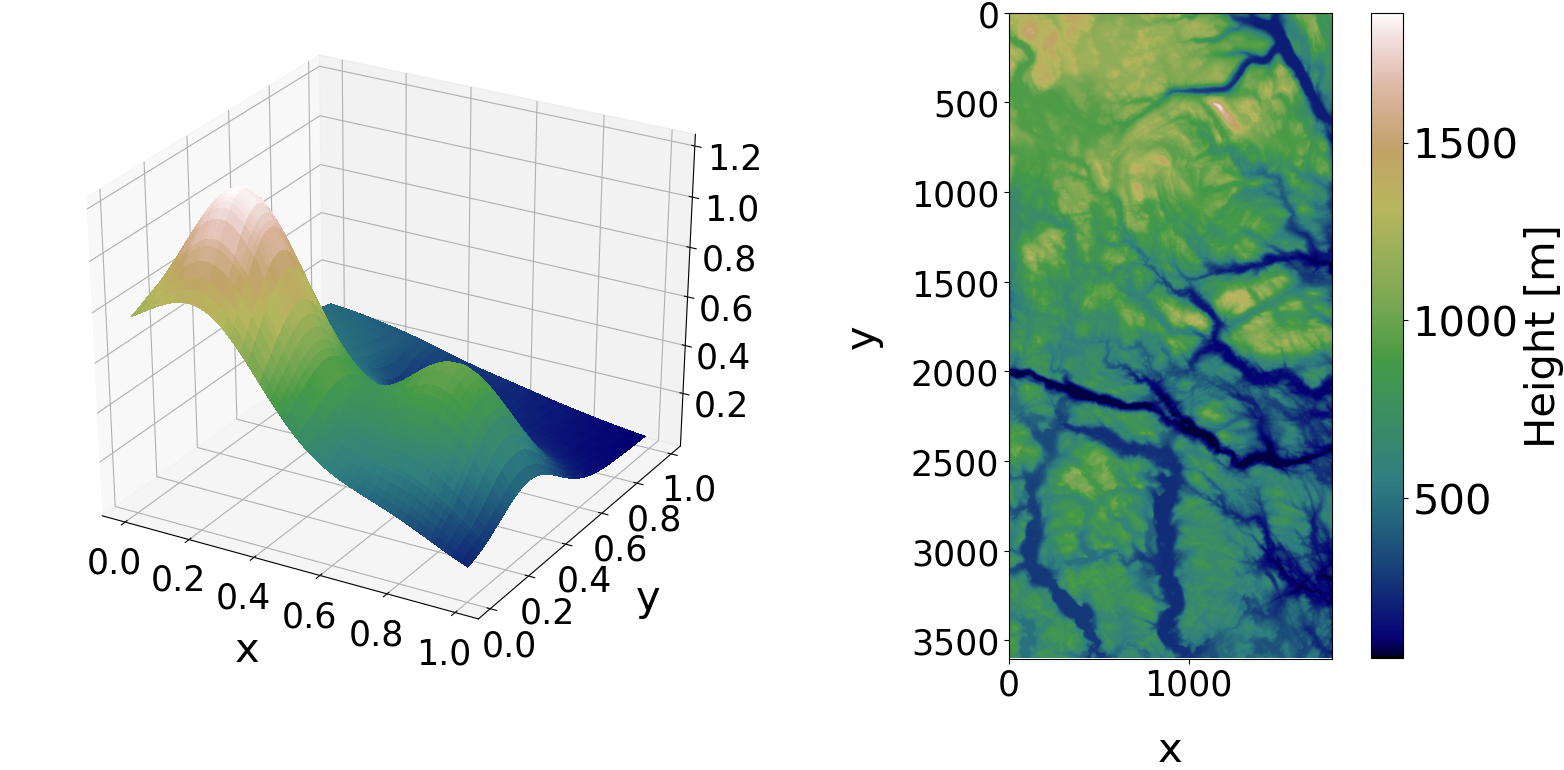
\includegraphics[width=\columnwidth]{Input_data.png}
  \caption{Data sets used as output (or dependant variables) for the linear regression. Franke function (left) and digital terrain data from Norwegian west coast (right).}
    \label{Input_data}
\end{figure}

The second dataset we analysed in this project is a digital terrain dataset from the west coast of Norway (see Figure \ref{Input_data} (right)). The data values vary between $50 m$ and $1865 m$ and it has a mean and standard deviation of $\sim703 m$ and $\sim303.5 m$, respectively. Therefore, we considered this dataset to be not well constrained and applied a scaling by dividing the data values with the maximum value of the dataset.

\subsection{Scaling}
When applying regression methods to find the optimal parameters $\mathbf{\beta}$, one has to take caution because the different column of the design matrix $\mathbf{X}$ (features) can have scales that are different order of magnitude. Scaling issues can have a big impact on the quality of the model fit, both in terms of the computational efficiency of fitting the model, and the quality of the estimates/predictions coming from the model. They also impact the interpretability of the estimates from the model. 

The design matrix to perform polynomial fitting of our dataset has the following form

\begin{align}
    \mathbf{X}= 
    \begin{bmatrix} 
    1 & x_0 & y_0 & x_0^2 & x_0 y_0 & y_0^2 & x_0^3 & \dots \\
    \\
    1 & x_1 & y_1  & y_1^2 & x_1 y_1   &  y_1^2  & x_1^3   & \dots \\
    \\
    \vdots & \vdots \\
    \\
    1 & x_{n-1} & y_{n-1} & x_{n-1}^2 & x_{n-1} y_{n-1} & y_{n-1}^2 & x_{n-1}^3 & \dots \\
    \end{bmatrix}.
    \label{_auto1} 
\end{align}

When scaling $\mathbf{X}$, one needs to treat the first column separately. This is to avoid assigning zeros in the first column as a result of centering of the design matrix. Scaling the design matrix may not be crucial for the OLS, but the tests we conducted using the Franke function shows that the two shrinkage methods (Ridge and LASSO) provide better results when $\mathbf{X}$ is scaled. The scaling we use here include centering by subtracting the mean and division with the standard deviation. The centering helps to avoid penalizing the intercept coefficient and the division with the standard deviation allows not to penalize unfairly the predictor variables are not on the same scale. Therefore, both the Franke function and the terrain data used in this project are analysed using a scaled design matrix.

\subsection{Data splitting}
In a machine learning  application, we expect our model not only to fit well to the history data, but also, and more importantly, performs an accurate prediction on the future data ("unseen" data). Therefore, we split the entire input data in to two parts which are the training dataset and the test dataset. In supervised learning, training dataset is labeled with known outputs (ground truth). As the name implies, training dataset is the subsection of the entire input data from which the model learns a certain pattern/operation to map the input into the output. Training data are also called in-sample. The error rate we get on the in-sample/training data by using error metric such as MSE or $R^2$ is therefore called in-sample error. Such a model performance metric evaluated using in-sample is retrodictive, not predictive. In contrast, test dataset is never used and should never be used for the training of the model. It is also called out-of-sample which provides a final estimate of the model’s performance after the training process. In order to optimally adjust the parameters of the model during the training process, a validation dataset can be generated. Here, the validation dataset is constructed by splitting the training dataset into a training and a validation data sets. We can then train our model on the new training dataset and estimate the performance on the validation dataset. 

\subsection{Resampling methods}
Resampling methods can be regarded as repetitive data splitting, that is to say we repeat the data splitting process multiple times and aggregate the results. Resampling is a good way to study model stability, allowing us to obtain additional information that would not be available from fitting the model only once using the original training samples \cite{lec}. It is especially useful for model assessment when the amount of input data is limited or when the data are not well behaved. Some of the most commonly used resampling methods are bootstrap and $k$-fold cross-validation. The difference between these two techniques is related to the way how to choose subsamples. 

\subsubsection*{Bootstrap}
Bootstrap is a flexible and powerful statistical tool. It can be used to analyze the uncertainty of parameter estimates quantitatively\cite{1986}. For example, it estimates the standard deviation of linear regression coefficients. The power of this method is that the concept is so simple that it can be easily applied to any model as long as the computational resource allows. The idea of empirical bootstrapping is to collect distinct data sets by repeatedly sampling observations from the original data set with replacement to create new bootstrapped data sets (Bootstrap samples) \cite{Pankaj}. Because these bootstrapped data sets are obtained by sampling with replacement, some observations may appear multiple times or not at all \cite{Kuhn}. In this project, Bootstrap is adopted when discussing the Bias-variances tradeoff and its working procedures can be summarized in Algorithm \ref{alg:bootstrap} as follows \cite{lec}:
\begin{algorithm}[H]
    \caption{Bootstrap}
    \label{alg:bootstrap}
    \begin{algorithmic}[1]
        \State Suppose we have a dataset with $M$ data points
        $\mathcal{D} = \{X_1,\ldots,X_M\}$.
        \State Split $\mathcal{D}$ into training $\mathcal{D}_{train}$ and testing $\mathcal{D}_{test}$.
        \For{i = 0, i < $N$ , i++}
            \State Randomly draw $M$ observations with replacement 
            $\mathcal{D}^{*(i)} = \{X_1^{*(i)},\ldots,X_M^{*(i)}\}$
            \State Fit $\mathcal{D}^{*(i)}$ to a given model.
            \State Evaluate the model on the $\mathcal{D}_{test}$ data or estimate the quantity of interest.
            \State Store relevant results.
        \EndFor
        \State Average on the stored results
    \end{algorithmic}
\end{algorithm}

\subsubsection*{$k$-fold cross-validation}
\label{kfold}
The $k$-fold cross-validation is a resampling method which works by first splitting the training data into $k$ equal sized parts (folds) and where the folds are different from each other. Often the number for $k$ is set to $5$ or $10$, but it can in principle be as large as the full data set size (i.e., leave-one-out cross-validation). One among the $k$ folds is then set as the validation dataset, and the model will be trained on the remaining $k-1$ folds. We repeat this procedure until every fold has been used once as the validation dataset and we can therefore get $k$ validation-errors if we apply error metrics every time. We then average the $k$ validation-errors and this is our estimate for the validation error. The procedure of using $k$-fold cross-validation is summarized in Algorithm \ref{alg:kfcv} as follows \cite{lec} \cite{hastie}:

\begin{algorithm}[H]
    \caption{$k$-fold Cross-validation}
    \label{alg:kfcv}
    \begin{algorithmic}[1]
        \State Shuffle the dataset randomly
        \State Split the dataset into $k$-folds
        \For{each unique fold}
            \State Take the fold as a hold out or validation data set
            \State Take the remaining $k-1$ folds as a training data set
            \State Fit a model on the training set and evaluate it on the validation set
            \State Retain the evaluation score and discard the model
        \EndFor
        \State Average the evaluation scores
    \end{algorithmic}
\end{algorithm}

\subsection{Error metrics}
The performance of a regression method is measured quantitatively using error metrics. In this project, we used the MSE and the $R^2$ score.

\subsubsection*{Mean squared error}

The most direct way to measure the performance of a model is to calculate the difference between the estimated value of the model and the actual data, sample-by-sample. The MSE is such an error metric often used for fitting of continuous functions. It calculates the average of the squared error. The larger the value of the MSE the poorer the performance of the model. MSE is mathematically defined as

\begin{equation}
    MSE = \frac{1}{n}
    \sum_{i=0}^{n-1}(y_i-\hat{y}_i)^2,
    \label{eq:MSE}
\end{equation}

where $y_i$ is the actual data value, $\hat{y_i}$ is the predicted data point, and $n$ is the total number of data samples.

\subsubsection*{$R^2$ score}

The $R^2$ score is a normalized error metric and its values vary between $0$ and $1$. $R^2$ represents the proportion of the variance in the dependent variable that is predictable from the independent variables. Mathematically, the $R^2$ score is given by

\begin{equation}
    R^2 = 1 - \frac{\sum_{i=0}^{n - 1} (y_i - \hat{y}_i)^2}{\sum_{i=0}^{n - 1} (y_i - \bar{\mathbf{y}})^2}.
    \label{eq:R2}
\end{equation}

where $\bar{\mathbf{y}}$ is the mean of $\mathbf{y}$. An $R^2$ score of $0$ means that the model is as accurate as the mean of the data and a negative score indicates that the mean is a better fit than the model.

\subsection{Implementation}
All the analysis in this project are implemented using Python programming language. The basic structure of our implementation includes a file \texttt{functions.py} containing all the necessary functions for performing regressions, resampling, and calculation of the error metrics. Then, using our two Jupyter notebooks for the Franke function \texttt{Franke-report.ipynb} and for the terrain data \texttt{Terrain-\\report.ipynb} we call the function we want to be used in our analysis. 

The OLS and Ridge regressions have analytical expressions for the determination of the optimal parameters (cf. Equations \ref{eqn_ols} and \ref{eqn_Ridge}) and their corresponding variances (cf. Equations \ref{eqn_ols_var} and \ref{eqn_Ridge_var}). Thus, we used the library \textbf{numpy} and selected the function \texttt{numpy.linalg.inv} to perform the inversion required in the determination of the OLS and Ridge regression optimal parameters and the corresponding confidence intervals. However, the LASSO regression does not have a closed form solution for the optimal parameters. Thus, we have used the LASSO regression provided by the library \textbf{Scikit-Learn}. To determine the confidence interval of the optimal parameters, we used the Bootstrap method first to estimate the variance of the optimal parameters and then computed the corresponding confidence intervals.

To perform $k$-fold cross-validation, we implemented a function named \texttt{k\_fold\_cv}. This function takes as input the number of $k$-folds, the output data (e.g., the Franke function or the terrain data), the design matrix, and the regression method of choice. This function then performs the $k$-fold cross-validation based on Algorithm \ref{alg:kfcv} and returns the $R^2$ and MSE metrics of the training and testing data sets.

\subsection{Unit tests}
Unit testing allows us to test the individual units of our source code to determine whether they are fit for use. We designed a unit test for fitting a second order polynomial function with known coefficients. We then performed regression using our implementation of the OLS and Ridge, and compared the result with that of the implementation from the library \textbf{Scikit-Learn}. We set a tolerance of $10^{-10}$ as the difference between the exact regression parameters $\boldsymbol{\beta}$ and our implementation. In addition, we also check our implementation of the error metrics against that of \textbf{Scikit-Learn}. All the unit tests were successful. 

\section{Results}
In this section we analyse the three linear regression methods (i.e., OLS, Ridge, and LASSO) using the numerically generated data, Franke function, and a digital topography data from the west of Norway.

\subsection{OLS regression on the Franke function}
Our task here is to explore linear regression methods for fitting the Franke function with polynomials of different order. We start our analysis by considering a noise free case and the OLS as our linear regression method. We selected three models to fit our data: (i) a $1^{st}$ order polynomial, which has three parameters, (ii) a $5^{th}$ order polynomial, which has $21$ parameters, and (iii) a $10^{th}$ order polynomial, which has $66$ parameters. We divided our dataset (size $165\times165$) into $training$ (size $132\times132$) and $testing$ (size $33\times33$), and learned the optimal regression parameters $\hat{\boldsymbol{\beta}}_{\text{OLS}}$ using the training dataset. The effectiveness of our model is then checked using the test dataset. Here, notice that to check the generalizing power of our models we made the range of the testing dataset to be between $0$ and $1.2$ while the training dataset is between $0$ and $1$. Figures \ref{NoiseFree_OLS_degree1}, \ref{NoiseFree_OLS_degree5}, and \ref{NoiseFree_OLS_degree10} show, respectively, the data fitting on the training dataset (on the left) and our prediction using the test dataset (on the right) for the $1^{st}$, $5^{th}$, and $10^{th}$ order polynomial models. As expected, given enough number of data samples the most complex model (i.e., $10^{th}$ order polynomial) fits the training data best. However, the $10^{th}$ order polynomial performs the worst in predicting the test dataset and especially for the region of the test dataset that is not in the range of the training dataset. Overall, we can see that it is difficult to generalize beyond the situations encountered in the training dataset and error in the test dataset exacerbates as the model gets very complex.

\begin{figure}
  \centering
  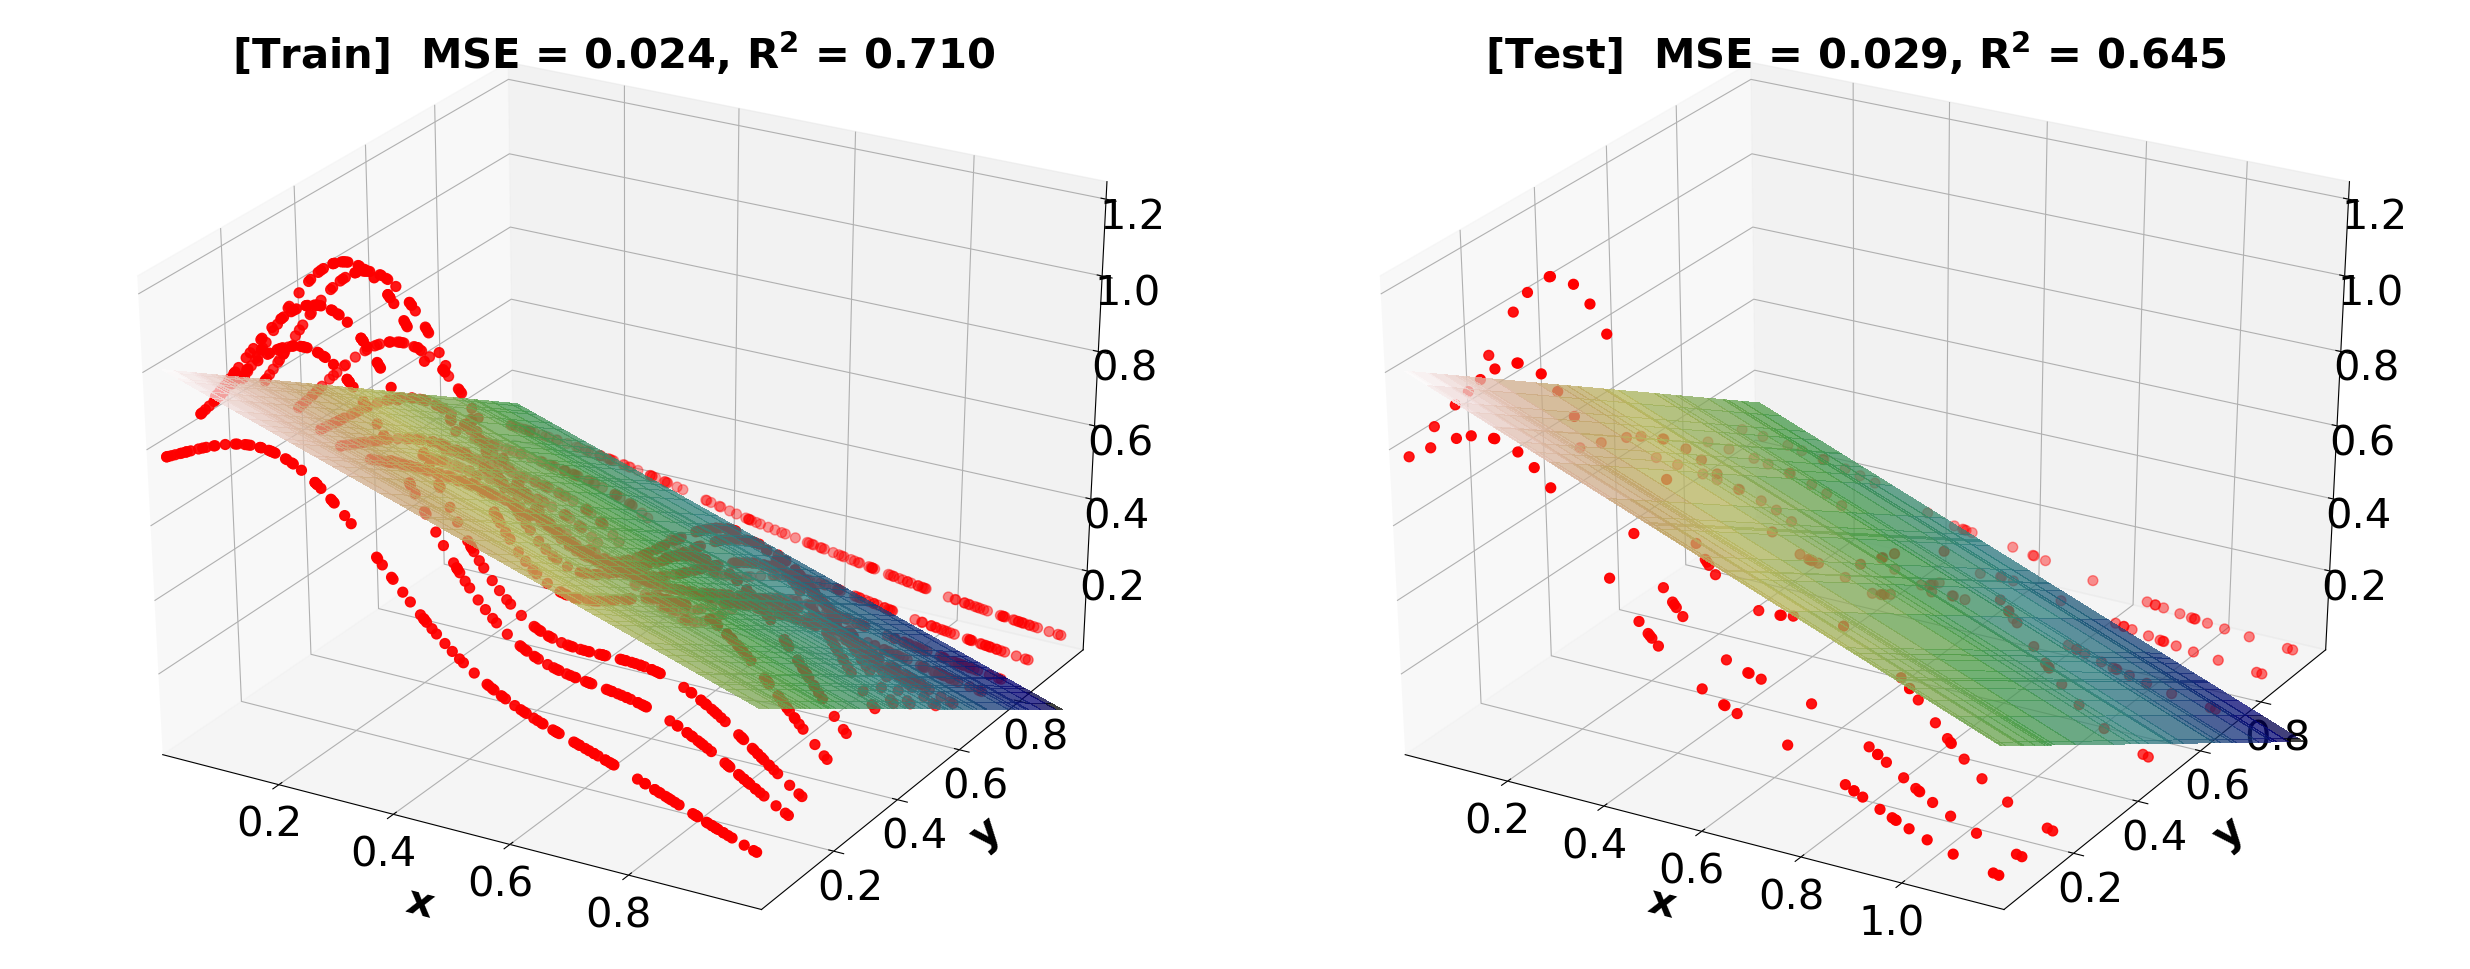
\includegraphics[width=\columnwidth]{NoiseFree_OLS_degree1.png}
  \caption{OLS fitting of the Franke function using $1^{st}$ order polynomial (left) and the corresponding prediction in the test data (right). The red dot scatter plot indicates the noise free Franke function data (every fifth data sample is plotted).}
    \label{NoiseFree_OLS_degree1}
\end{figure}
\begin{figure}
  \centering
  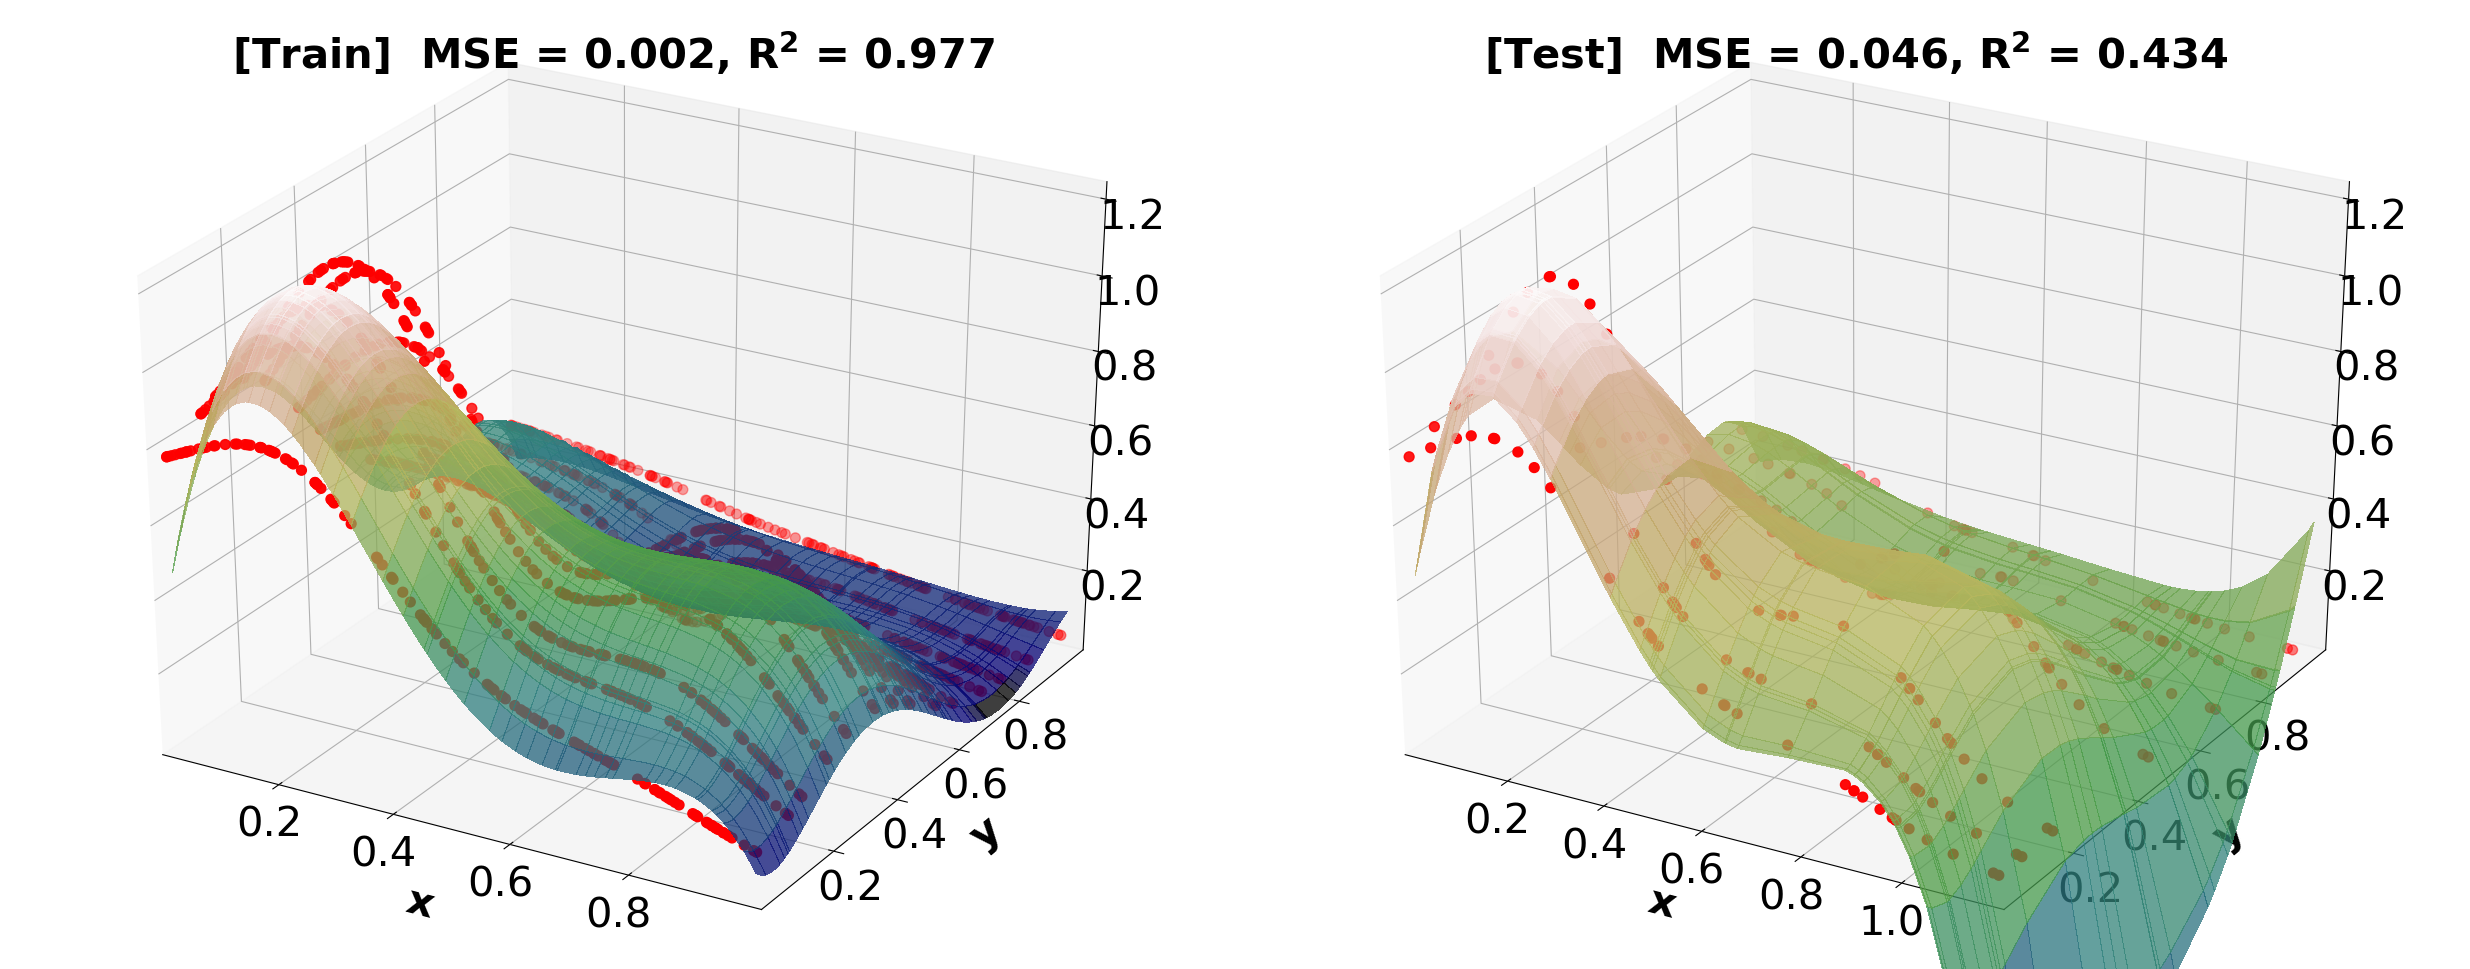
\includegraphics[width=\columnwidth]{NoiseFree_OLS_degree5.png}
  \caption{OLS fitting of the Franke function using $5^{th}$ order polynomial (left) and the corresponding prediction in the test data (right). The red dot scatter plot indicates the noise free Franke function data (every fifth data sample is plotted).}
    \label{NoiseFree_OLS_degree5}
\end{figure}
\begin{figure}
  \centering
  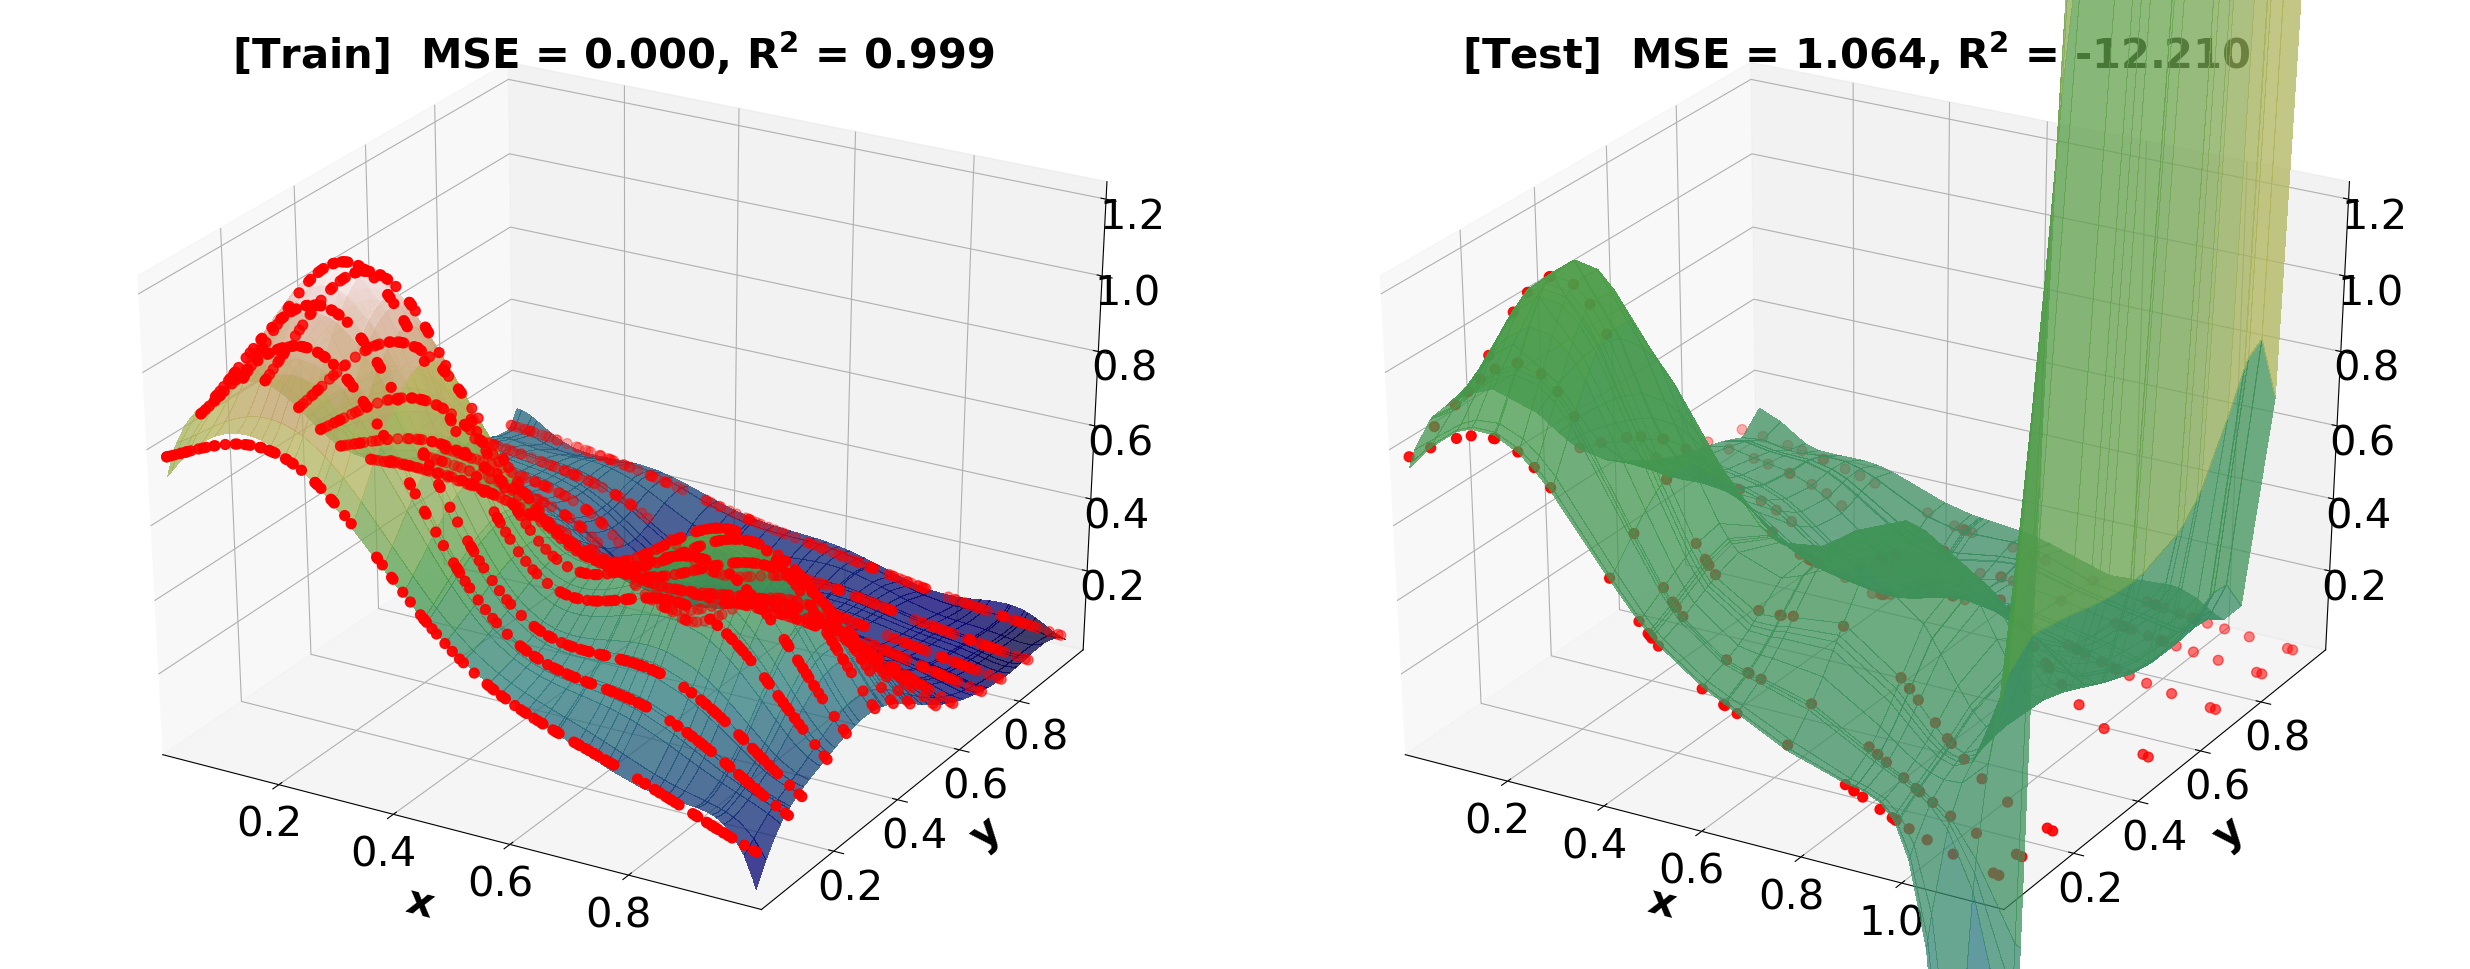
\includegraphics[width=\columnwidth]{NoiseFree_OLS_degree10.png}
  \caption{ OLS fitting of the Franke function using $10^{th}$ order polynomial (left) and the corresponding prediction in the test data (right). The red dot scatter plot indicates the noise free Franke function data (every fifth data sample is plotted).}
    \label{NoiseFree_OLS_degree10}
\end{figure}

We now add noise to our dataset. The noise has Gaussian distribution with zero mean and variance of $\sigma_{\epsilon}^2$, where $\sigma_{\epsilon}$ is $10\%$ of the maximum absolute value of the Franke function. Here, again we divided our dataset into training and testing, and applied the three polynomial models we used for the noise free case. Figures \ref{Noisy_OLS_degree1}, \ref{Noisy_OLS_degree5}, and \ref{Noisy_OLS_degree10} show that all the three models perform worse than their noise free case counterparts. However, the most complex model, the $10^{th}$ order polynomial, produced the best fit to the training dataset while giving the worst prediction on the test dataset. Therefore, when the given number of data samples are not large enough, simpler models (e.g., $1^{st}$ and $5^{th}$ order polynomials) are better at prediction than complex
models (e.g., $10^{th}$ order polynomial). This is mainly due to the bias-variance tradeoff, where the simpler models have high bias but less variance, and the complex models have less bias but high variance. The consequence of having a high variance but low bias is that the model will result in overfitting which substantially degrades the predictive performance on the test data.

\begin{figure}[H]
  \centering
  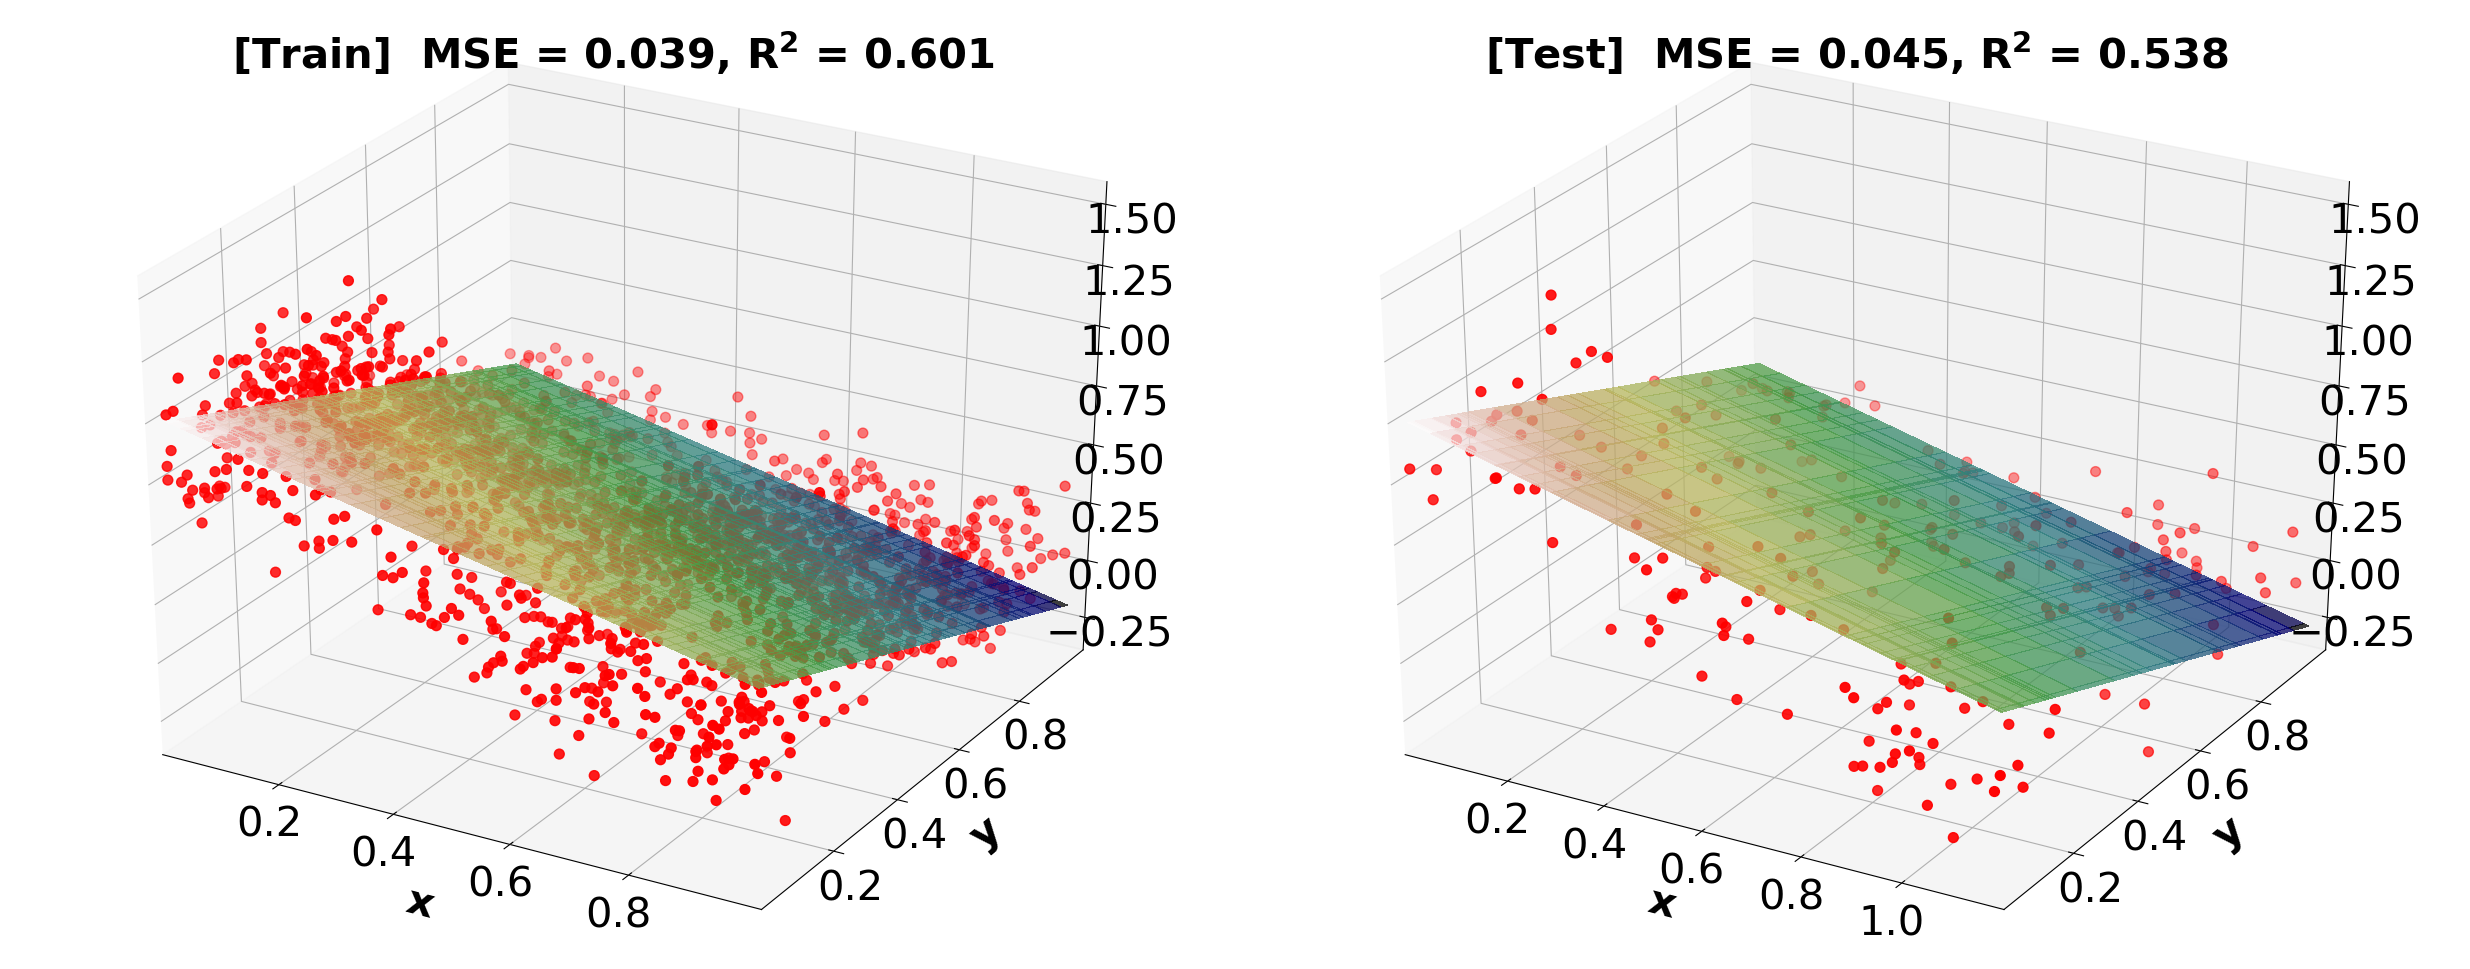
\includegraphics[width=\columnwidth]{Noisy_OLS_degree1.png}
  \caption{OLS fitting of the Franke function using $1^{st}$ order polynomial (left) and the corresponding prediction in the test data (right). The red dot scatter plot indicates the noise contaminated Franke function data (every fifth data sample is plotted).}
    \label{Noisy_OLS_degree1}
\end{figure}
\begin{figure}[H]
  \centering
  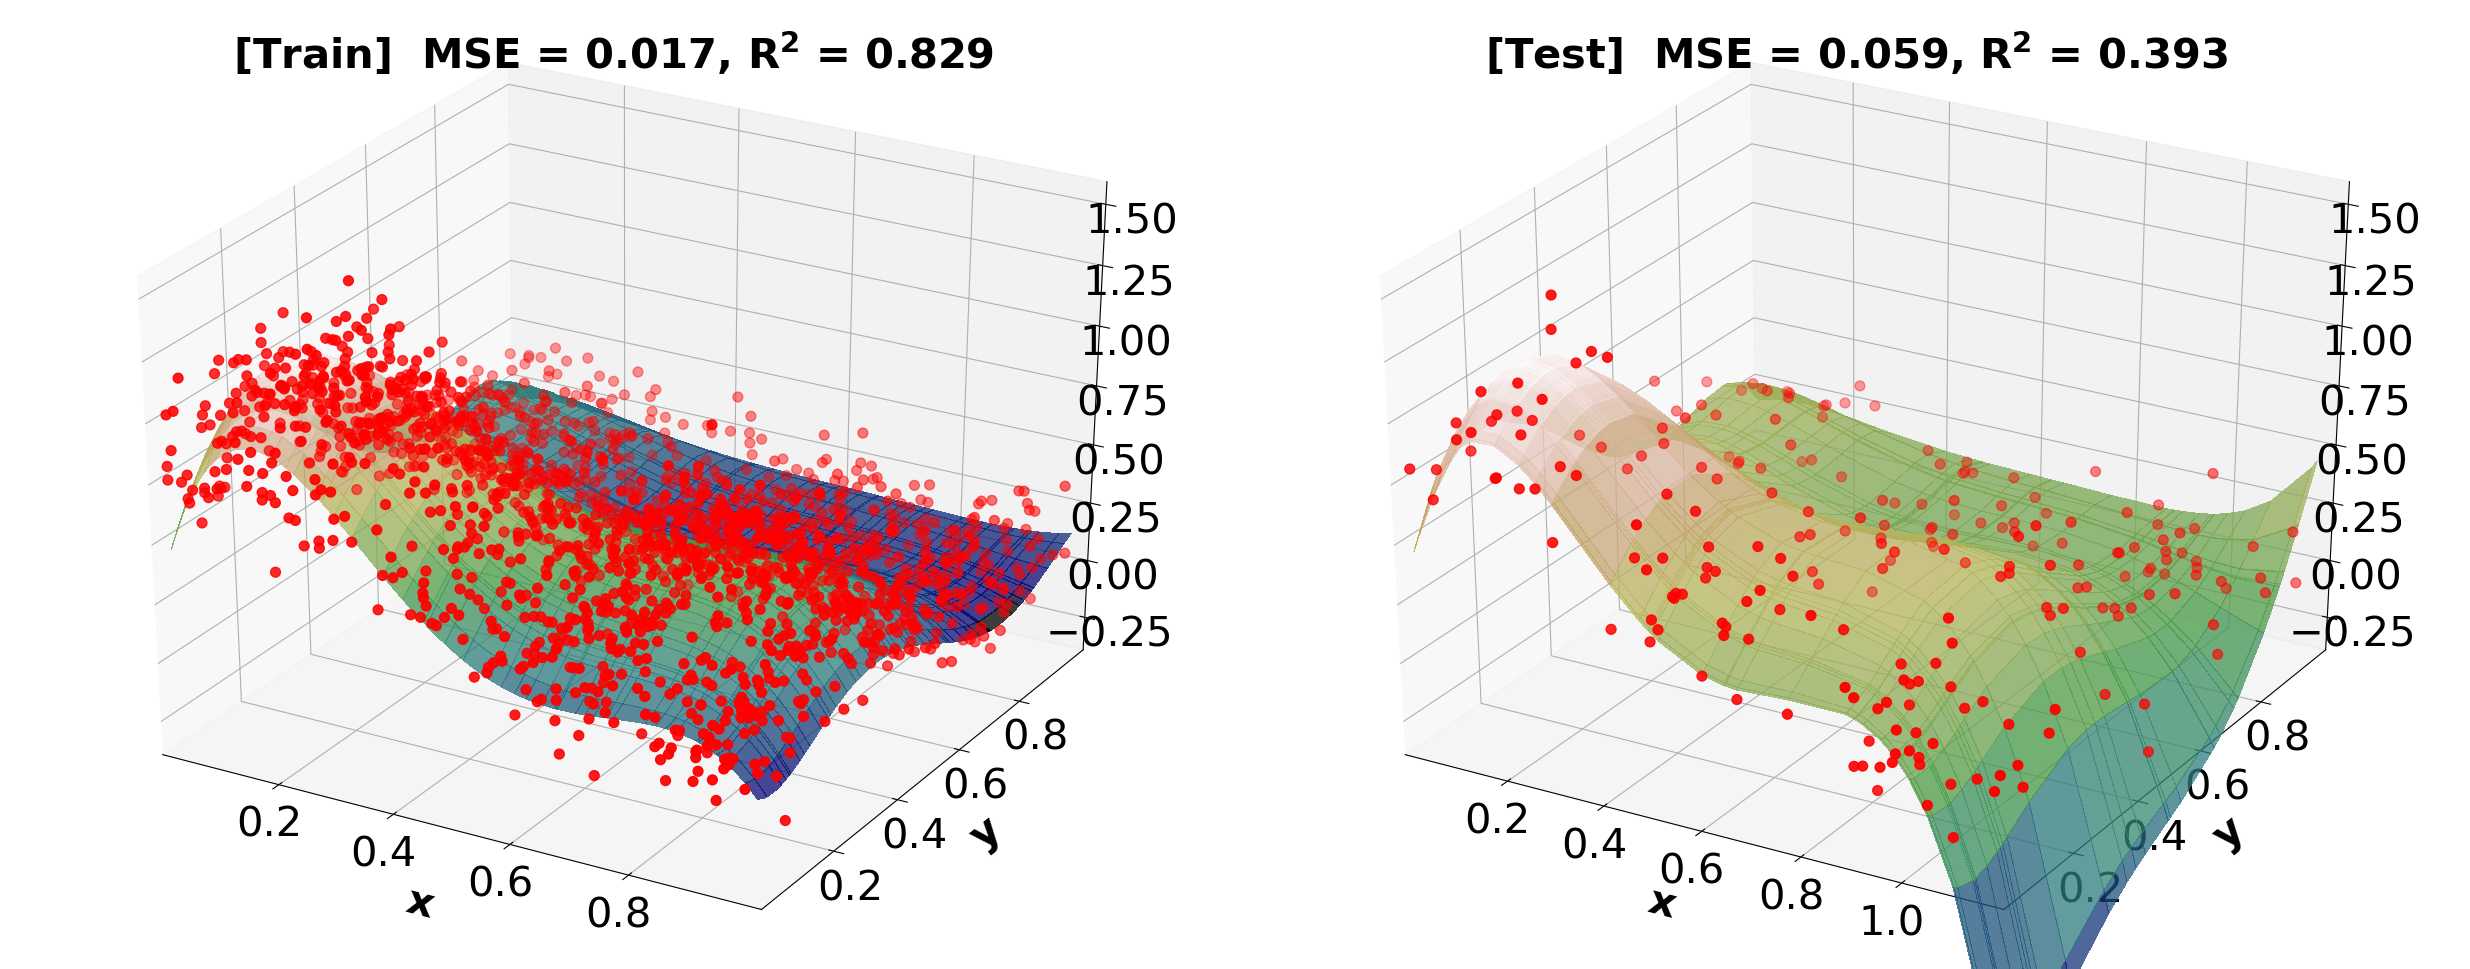
\includegraphics[width=\columnwidth]{Noisy_OLS_degree5.png}
  \caption{OLS fitting of the Franke function using $5^{th}$ order polynomial (left) and the corresponding prediction in the test data (right). The red dot scatter plot indicates the noise contaminated Franke function data (every fifth data sample is plotted).}
    \label{Noisy_OLS_degree5}
\end{figure}
\begin{figure}[H]
  \centering
  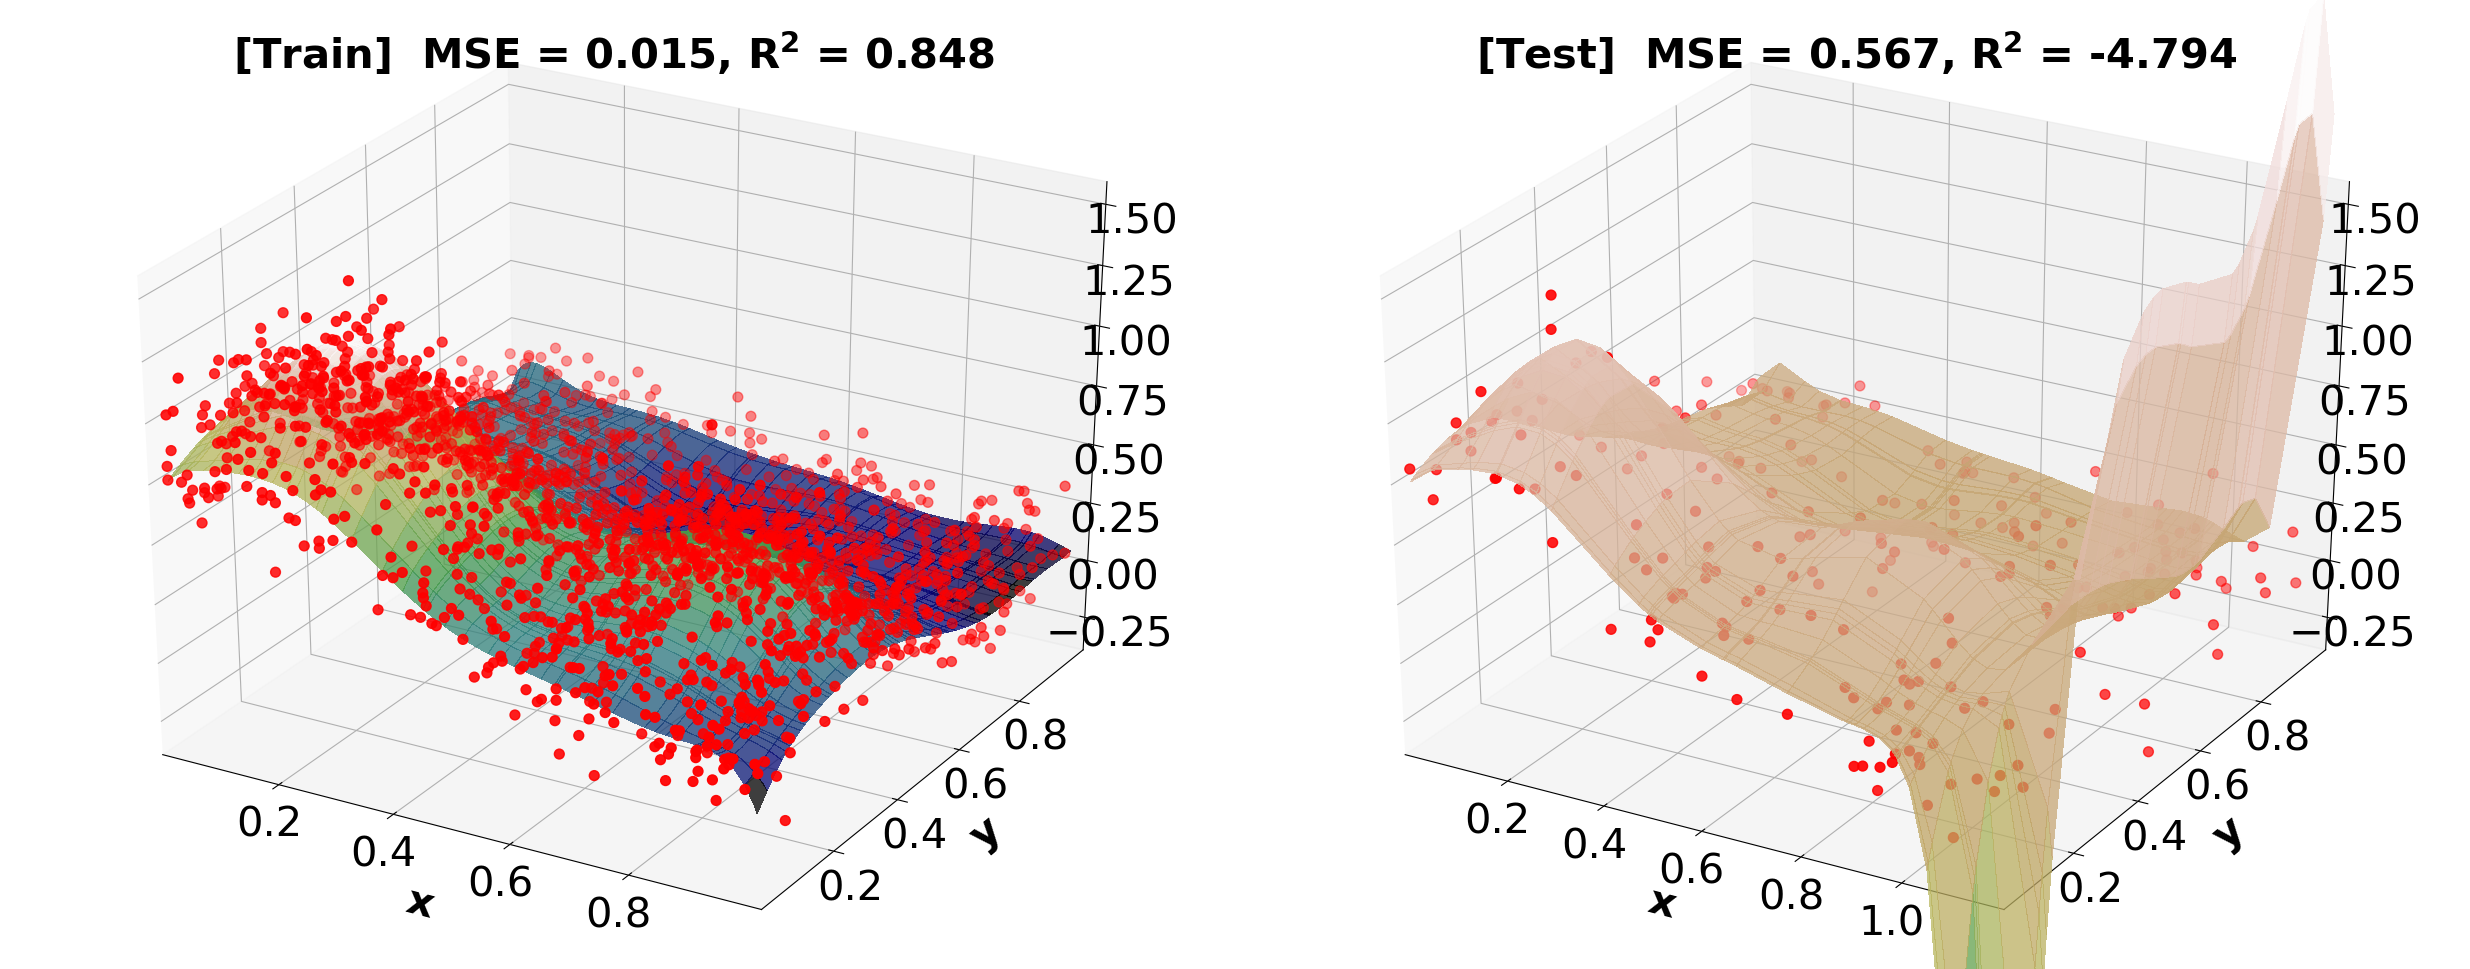
\includegraphics[width=\columnwidth]{Noisy_OLS_degree10.png}
  \caption{OLS fitting of the Franke function using $10^{th}$ order polynomial (left) and the corresponding prediction in the test data (right). The red dot scatter plot indicates the noise contaminated Franke function data (every fifth data sample is plotted).}
    \label{Noisy_OLS_degree10}
\end{figure}

To analyse the bias-variance tradeoff for our model we used the Bootstrap method and calculated the test data MSE, bias, and variance for different models with different orders of polynomial. We have used $113$ bootstraps and our models vary from $0^{th}$ to $12^{th}$ order polynomial. Notice, for all the polynomial orders we have enough number of training samples to fit the parameters. In general, simpler models (i.e., less than $4^{th}$ order polynomial) have high bias and low variance and thus these models pay very little attention to the training data and they result in underfitting. However, models higher than $11^{th}$ order polynomial have high variance and low bias and pay a lot of attention to the training data and does not generalize on the data which it has not seen before (see Figure \ref{Bias_varience_OLS}). 
\begin{figure}[H]
  \centering
  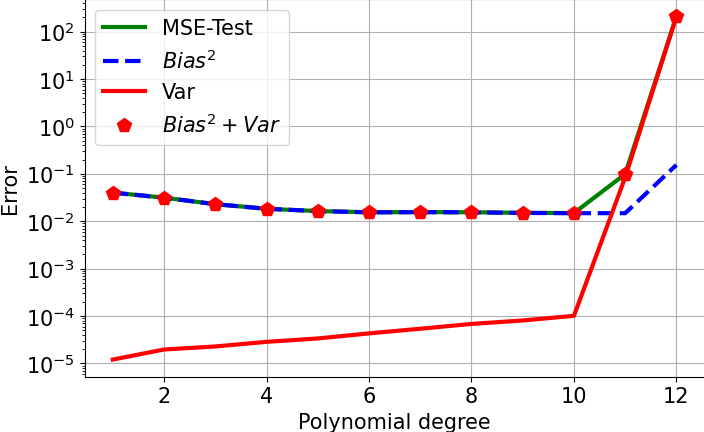
\includegraphics[width=4in,keepaspectratio]{Bias_varience_OLS.png}
  \caption{The bias-variance tradeoff for a Franke function with noise. The training/test split was set to $80/20$ and $113$ bootstrap iterations are used.}
    \label{Bias_varience_OLS}
    
\end{figure}
\begin{figure}[H]
  \centering
  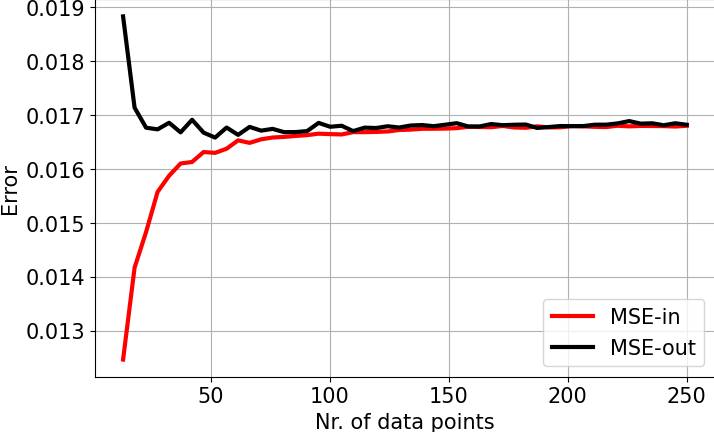
\includegraphics[width=4in,keepaspectratio]{Bias_varience_OLS_Nsamp.png}
  \caption{The in-sample and out-of-sample
errors for a polynomial order $5$ as a function of training data sizes. The errors were computed by generating random uniformly distributed samples in  $50$ different trails, and training for each trial and averaging the result.}
    \label{Bias_varience_OLS_nsamp}
\end{figure}

Figure \ref{Bias_varience_OLS_nsamp}, shows for a $5^{th}$ order polynomial model, the out-of-sample and in-sample errors as a function of the amount of training data. Here, it is possible to see that when the number of training data gets larger, the in-sample error increases and the out-off-sample error decreases while they both reach a plateau around an error value of $0.0168$, which corresponds to the “bias” of our model.

The optimal model for our problem of fitting and predicting the Franke function can be obtained by using the $k$-fold cross-validation technique. Here, we use a $5$-fold cross-validation and computed both the training and testing MSE and $R^2$ sores. Figure \ref{Modelsel_OLS} shows both the MSE and $R^2$ sores are flat for polynomial orders between $7$ and $10$. Therefore, for the OLS regression on the noisy Franke function, we selected polynomial order of $7$ to be the optimal model.

\subsection{Ridge and LASSO regressions on the Franke function}
The OLS allows a high variance in the estimator coefficients $\mathbf{\beta}$, which can lead to overfitting. Therefore, we consider two shrinkage methods to remedy this issue, namely the Ridge and LASSO regression methods. To see the advantages of the shrinkage methods in overcoming overfitting problem, we applied the Ridge and LASSO regressions on the noisy Franke function (see Figures \ref{Noisy_Ridge_degree10} and \ref{Noisy_LASSO_degree10}). A $10^{th}$ order polynomial model is used for the regressions and hyper-parameters are set to $0.1$ for Ridge and $0.001$ for LASSO. Comparing the results of Figures \ref{Noisy_OLS_degree10}, \ref{Noisy_Ridge_degree10}, and \ref{Noisy_LASSO_degree10}, we can see that the two shrinkage methods have smaller test MSE, better prediction, than the OLS result. However, the two shrinkage methods sacrificed the fitting of the training data, higher training MSE. 

\begin{figure}[H]
  \centering
  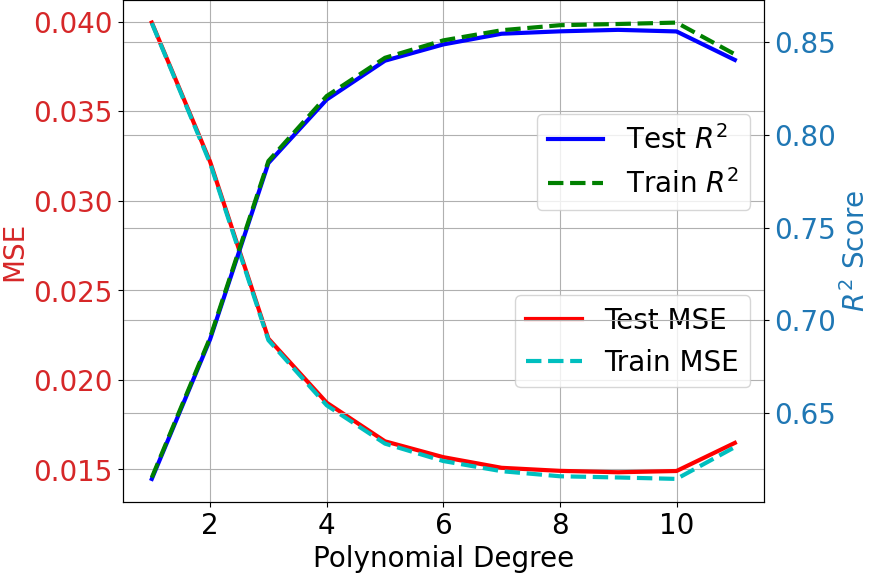
\includegraphics[width=4in,keepaspectratio]{Modelsel_OLS.png}
  \caption{Performance of the OLS regression on the noisy Franke function measured by the train and test MSE and $R^2$ sore.}
    \label{Modelsel_OLS}
\end{figure}

\begin{figure}[H]
  \centering
  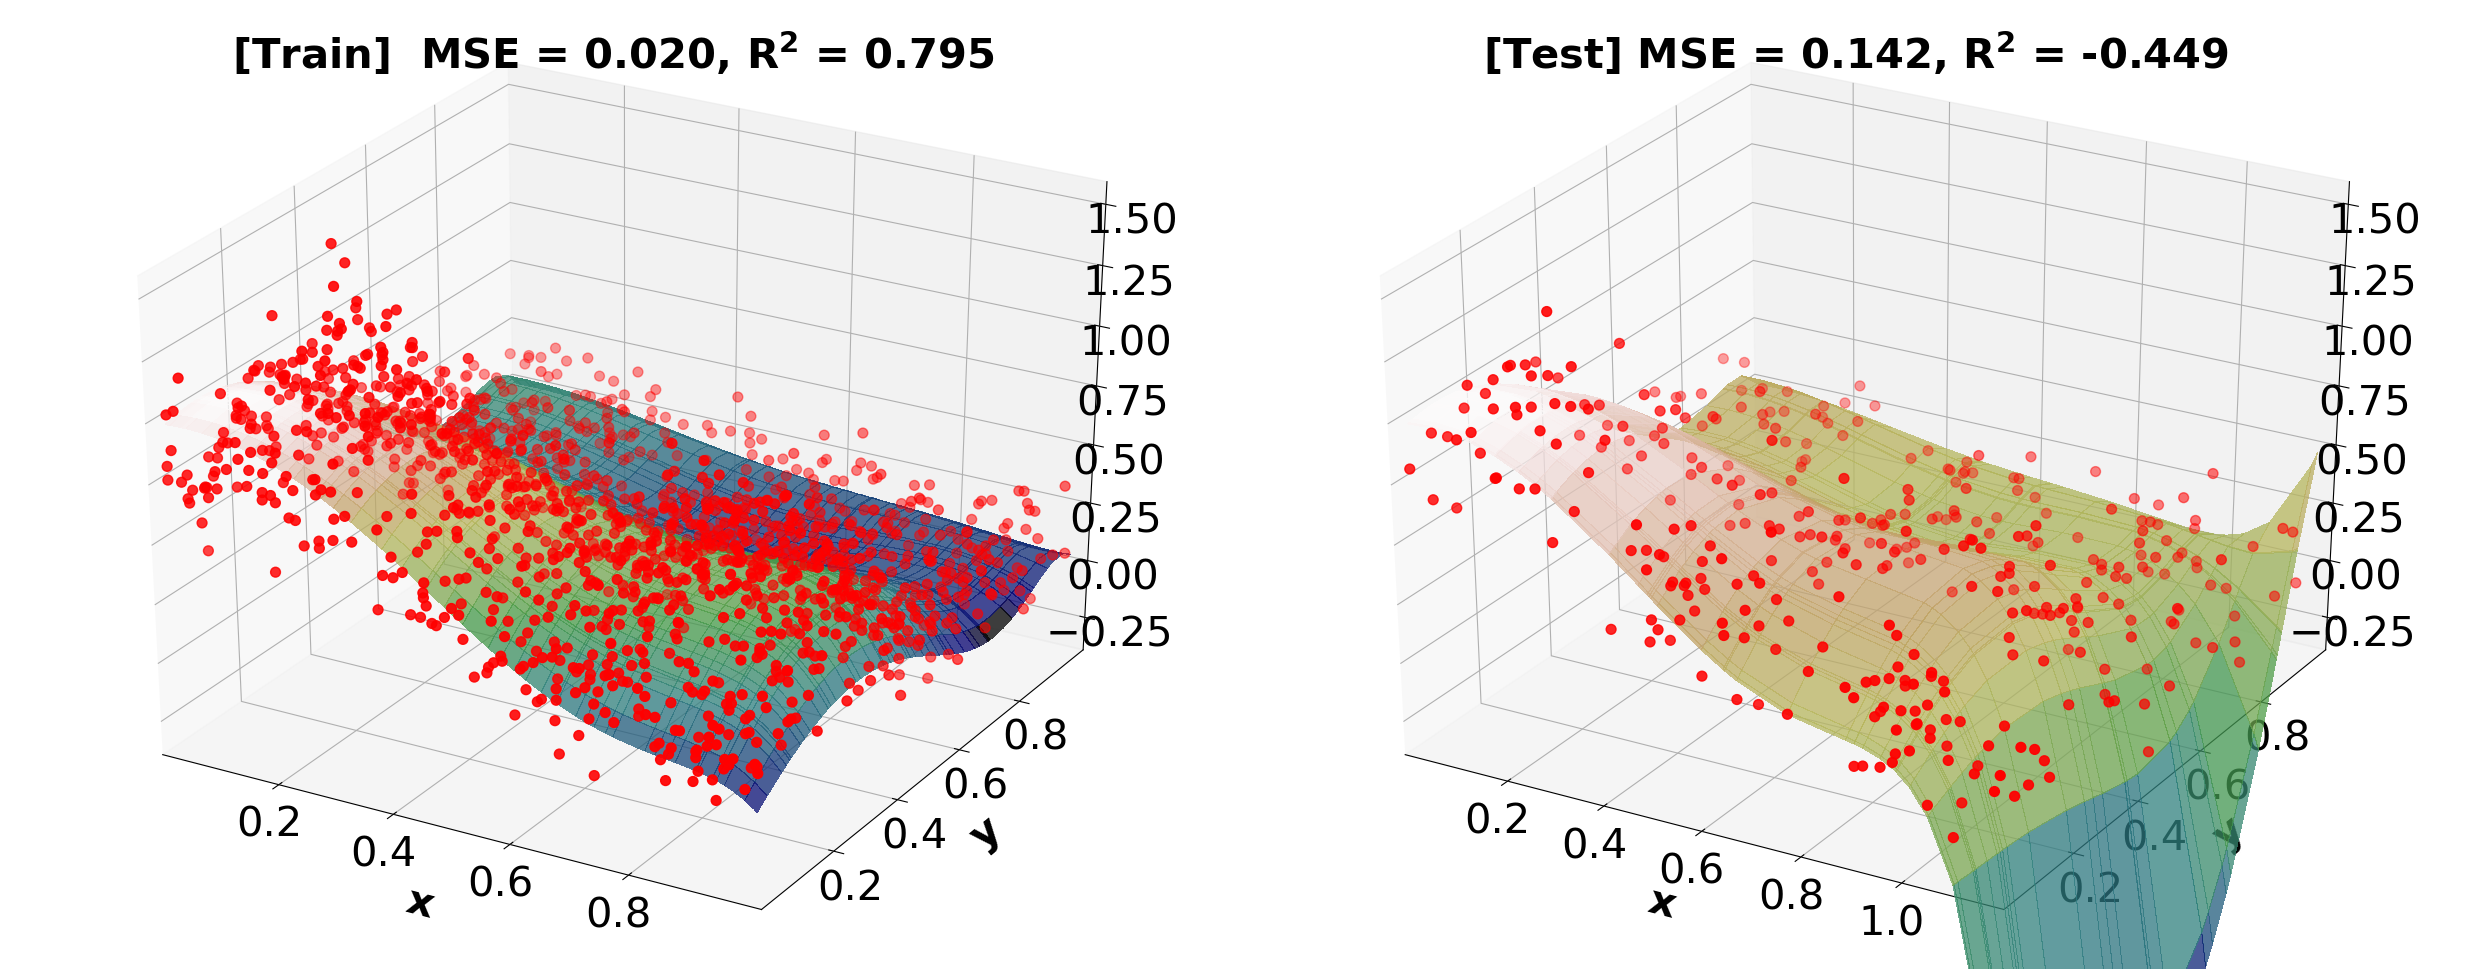
\includegraphics[width=\columnwidth]{Noisy_Ridge_degree10.png}
  \caption{Ridge regression fitting of the Franke function using $10^{th}$ order polynomial (left) and the corresponding prediction in the test data (right). The red dot scatter plot indicates the noise contaminated Franke function data (every fifth data sample is plotted).}
    \label{Noisy_Ridge_degree10}
\end{figure}
\begin{figure}
  \centering
  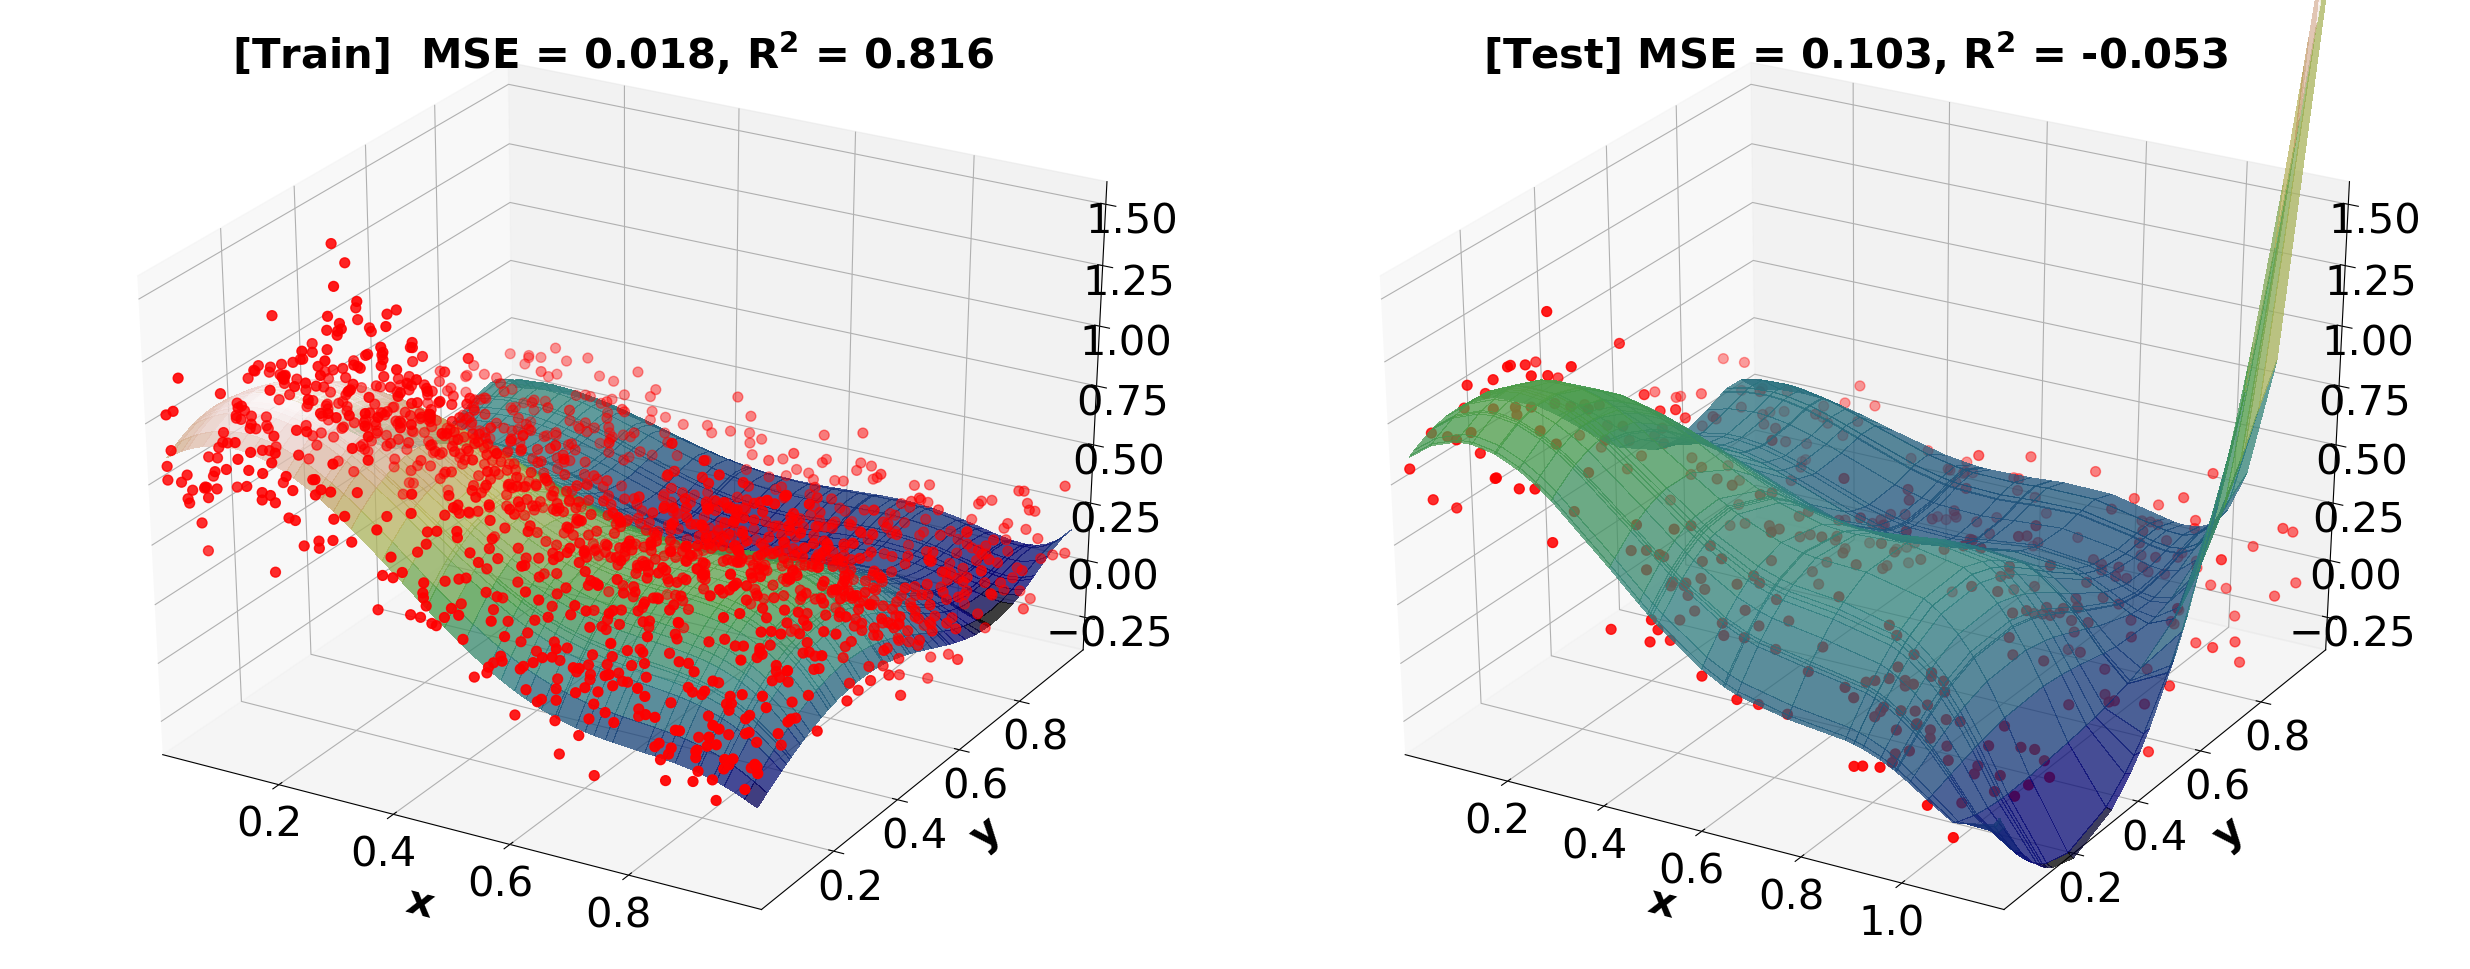
\includegraphics[width=\columnwidth]{Noisy_LASSO_degree10.png}
  \caption{LASSO regression fitting of the Franke function using $10^{th}$ order polynomial (left) and the corresponding prediction in the test data (right). The red dot scatter plot indicates the noise contaminated Franke function data (every fifth data sample is plotted).}
    \label{Noisy_LASSO_degree10}
\end{figure}

Finding the balance between a good fitting of the training data and a better prediction of the test data is a crucial element of any shrinkage method. Therefore, for the Ridge and LASSO regressions, using $5$-fold cross validation we searched for the optimal models and their corresponding hyper-parameters (see Figure \ref{Bias_varienceRidge_LASSO_lambda}). From Figure \ref{Bias_varienceRidge_LASSO_lambda} we can see that for the Ridge regression the smallest test MSE is achieved with a polynomial order of $8$ and $\lambda=10^{-6}$. For LASSO regression we notice that the test MSE in the range between $7$ and $11$ polynomial orders is approximately the same when $\lambda=10^{-5}$. Therefore, we selected polynomial order of $7$ to be the optimal model for the LASSO regression. However, it is pertinent to note that due to shortage of computational resources, we have not tested the LASSO regression for $\lambda < 10^{-5}$.

\begin{figure}[ht]
     \centering
     \begin{subfigure}{.475\textwidth}
         \centering
         \includegraphics[width=1\linewidth]{Modelsel_Ridge_scaled.png}
     \end{subfigure}
     \begin{subfigure}{.475\textwidth}
         \centering
         \includegraphics[width=1\linewidth]{Modelsel_LASSO_scaled.png}
     \end{subfigure}
    \caption{Performance of the Ridge (left) and LASSO (right) regressions on the noisy Franke function as a function of the hyper-parameter $\lambda$ and the polynomial order and measured by the test MSE. }
    \label{Bias_varienceRidge_LASSO_lambda}
\end{figure}

The hyper-parameter $\lambda$ for the two shrinkage methods control the  bias-Variance tradeoff curve. Moreover, computing the bias-Variance tradeoff for different $\lambda$ allows us to make the decision between the fitting of the training data versus the size of the estimator coefficients $\mathbf{\beta}$. From Figure \ref{Bias_varienceRidge_LASSO_lambda2} we see that for both Ridge and LASSO, when $\lambda$ becomes very large, the bias stays unchanged and the variance continue to reduce. Therefore, Ridge and LASSO, with large $\lambda$ reduce the variance at the expense of larger bias and MSE.

\begin{figure}[ht]
     \centering
     \begin{subfigure}{.475\textwidth}
         \centering
         \includegraphics[width=1\linewidth]{Bias_varience_Ridge_lambda.png}
     \end{subfigure}
     \begin{subfigure}{.475\textwidth}
         \centering
         \includegraphics[width=1\linewidth]{Bias_varience_LASSO_lambda.png}
     \end{subfigure}
    \caption{The bias-variance curve as a function of the hyper-parameter $\lambda$ for Ridge (left) and LASSO (right) regressions.}
    \label{Bias_varienceRidge_LASSO_lambda2}
\end{figure}

If $\lambda=0$ then both the Ridge and LASSO regressions result in the same $\mathbf{\beta}$ coefficients as that of the OLS. However, when  $\lambda$ approaches to infinity, the impact of shrinkage penalty increases and the result of the Ridge and LASSO regressions estimator coefficients $\mathbf{\beta}$ will approach to zero (for LASSO the coefficients actually become zero) (see Figure \ref{Optimal_beta}). The advantage of shrinking the estimator coefficients $\mathbf{\beta}$ towards zero is that it allows us to reduce the non-impactful features and it saves the model from high variance with a stable fit.

Finally, we examine the fitting and predictions of the three regression methods when using the optimal model and the corresponding hyper-parameters. Figure \ref{OLS_Ridge_LASSO_degree} show the fitting and predictions measured using MSE and $R^2$ scores. For the training data, the Ridge regression has the best fitting performance (the $R^2$ score is slightly higher than the OLS), while on the testing data both the OLS and Ridge regression perform the same and they out perform the LASSO regression. Nevertheless, Figure \ref{Confidence_interval} show the optimal regression parameters $\hat{\mathbf{\beta}}$ for the OLS, Ridge, and LASSO regressions when using the optimal model and hyper-parameters. The corresponding $95\%$ confidence interval is also shown for each of the regression results. Notice, the confidence intervals for the OLS and Ridge have analytical expressions while for the LASSO we used $113$ bootstraps to determine the confidence interval. The optimal regression parameters $\hat{\mathbf{\beta}}$ for the LASSO regression are very small compared to the OLS and Ridge regression. This is because the optimal hyper-parameter ($\lambda=10^{-5}$) for the LASSO regression is large enough and consequently shrank the parameters.

\begin{figure}[H]
  \centering
  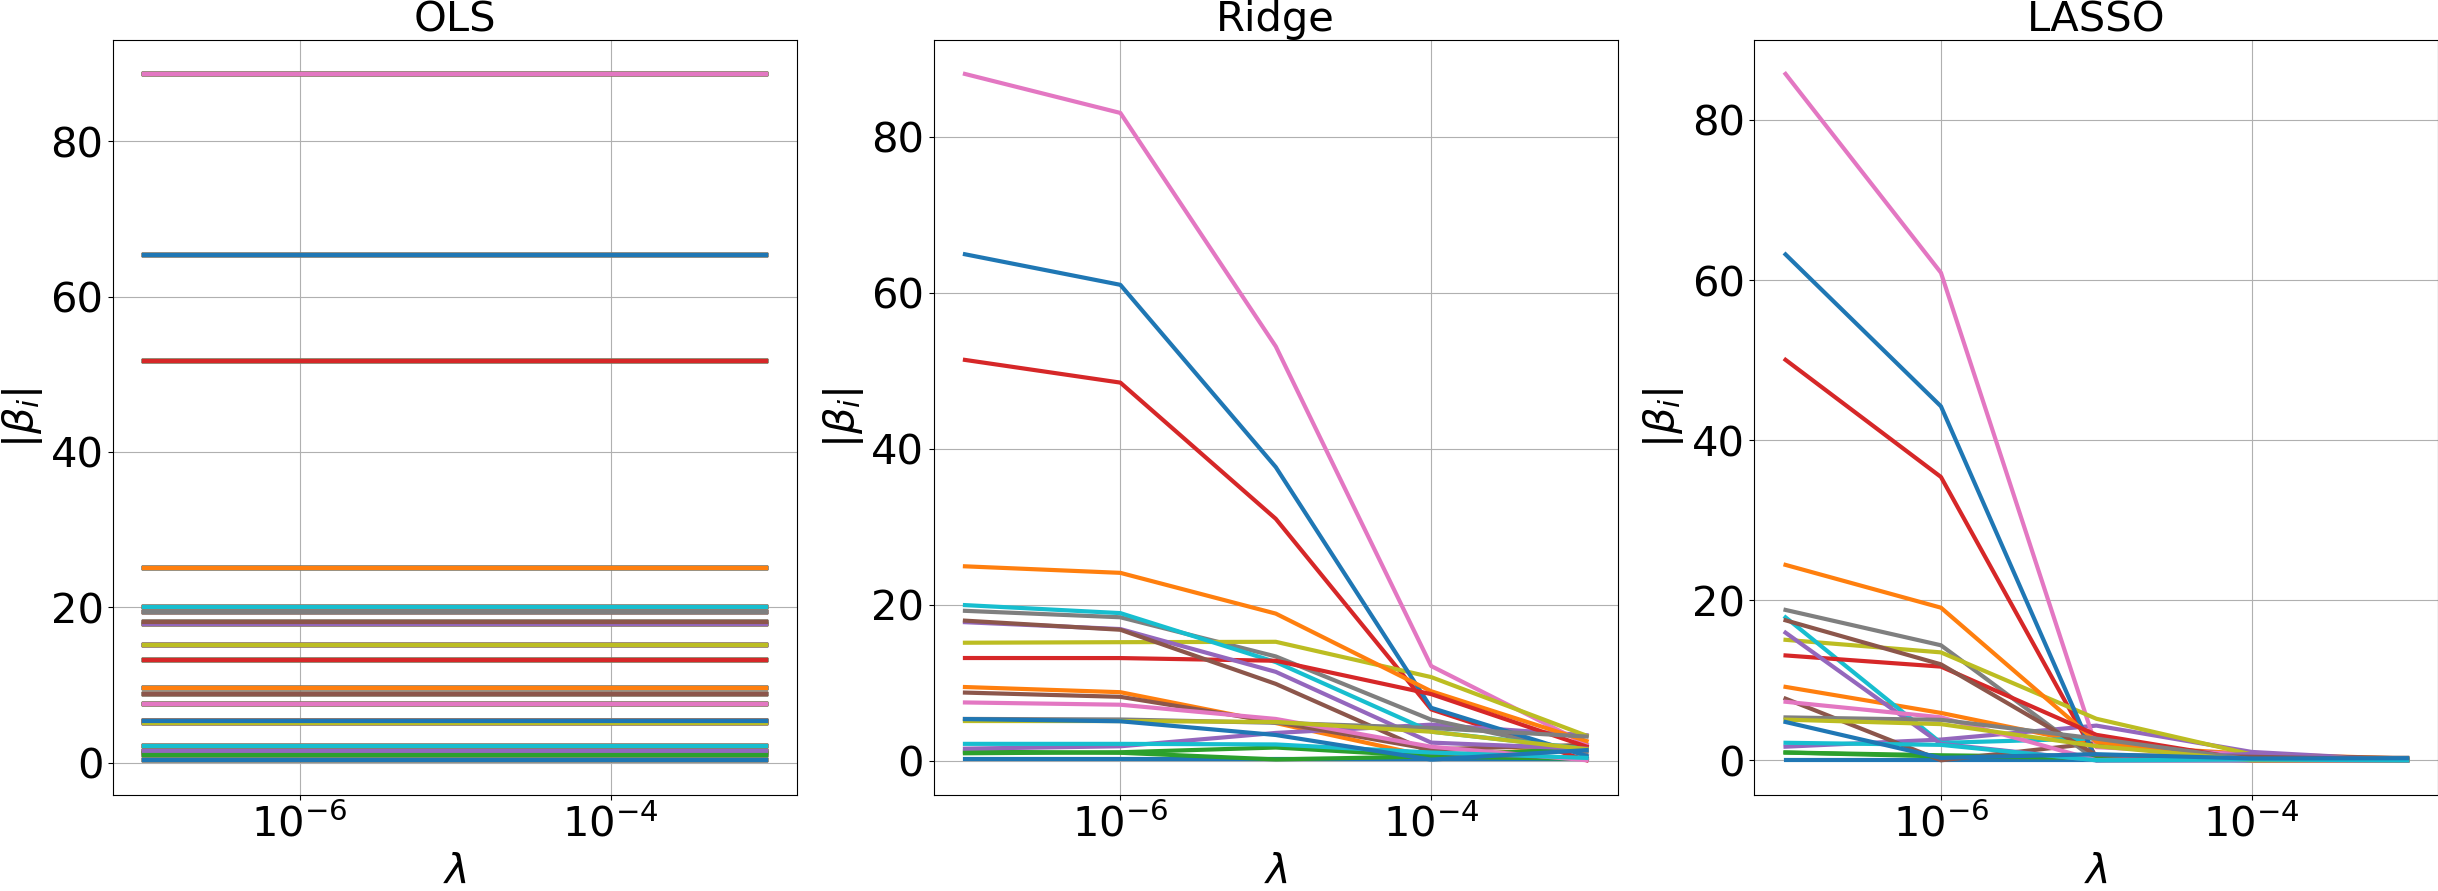
\includegraphics[width=\columnwidth]{Optimal_beta_scaled.png}
  \caption{The regularization path for the OLS (left), Ridge (middle), and LASSO (right) regressions on the noisy Franke function. Curves with different colors correspond to different coefficients $\mathbf{\beta}$. Notice LASSO, unlike Ridge, sets feature weights to zero leading to sparsity.}
    \label{Optimal_beta}
\end{figure}

\begin{figure}[H]
  \centering
  \includegraphics[width=\columnwidth]{OLS_Ridge_LASSO.png}
  \caption{The fitting (top row) and prediction (bottom row) performance of the OLS, Ridge, and LASSO regressions on the noisy Franke function.}
    \label{OLS_Ridge_LASSO_degree}
\end{figure}


\begin{figure}[H]
  \centering
  \includegraphics[width=\columnwidth]{Confidence_interval_scaled_new.png}
  \caption{The optimal regression parameters $\mathbf{\beta}$ for the OLS (left), Ridge (middle), and LASSO (right) on the noisy Franke function. The $95\%$ confidence interval is also shown. Notice, the polynomial order for the OLS, Ridge, and LASSO are $7$, $8$, and $7$, respectively.}
    \label{Confidence_interval}
\end{figure}

\subsection{Terrain dataset}
This dataset consists of $3601\times1801$ data points. This is a very large dataset to process in a single personal computer, hence we selected a small portion of this data set (see Figure \ref{Input_data_Terrain}(right)). The small portion has a size of $100\times100$. We start our analysis by normalizing the dataset so that the values vary between $0$ and $1$.
\begin{figure}
  \centering
  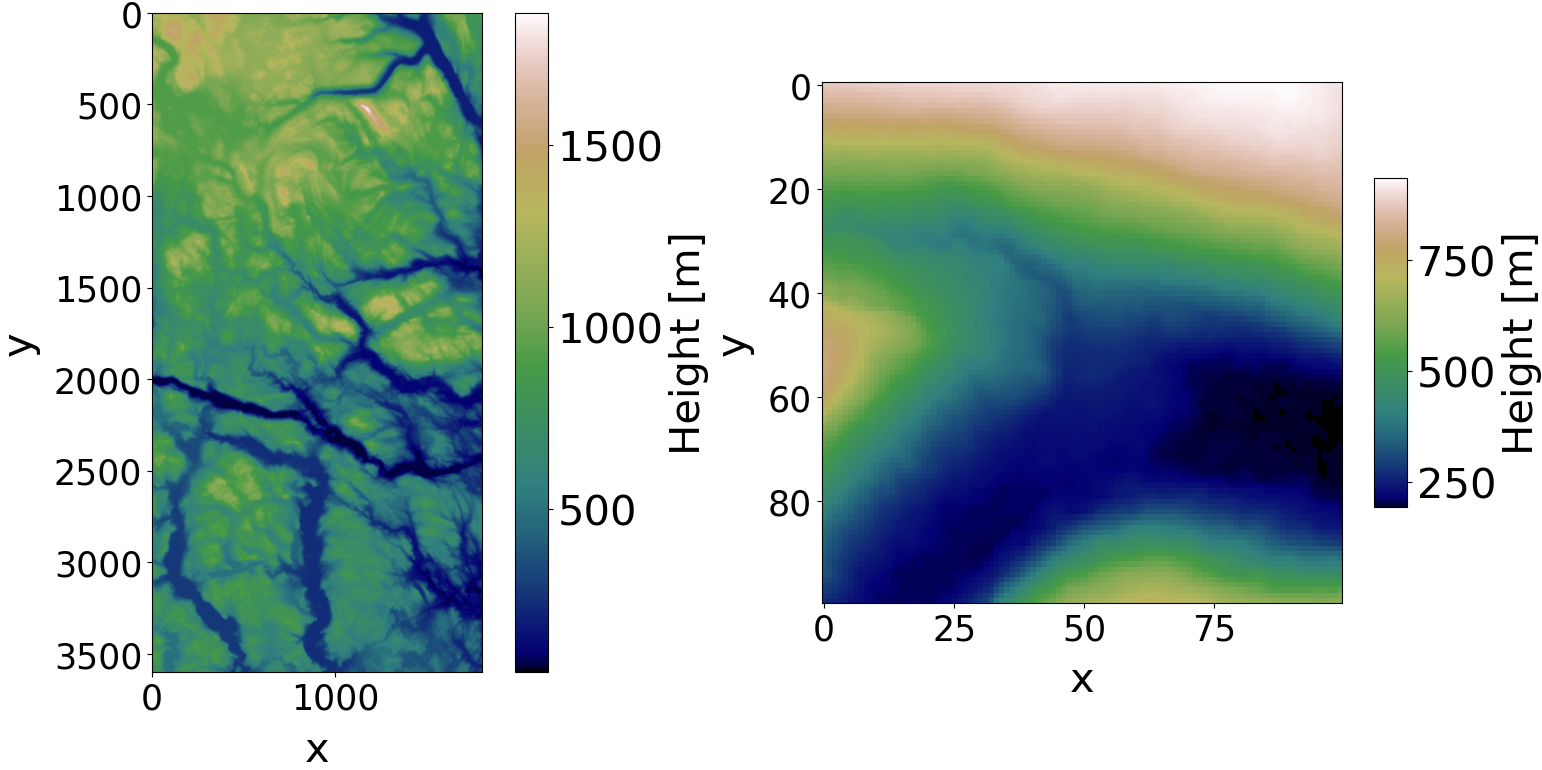
\includegraphics[width=\columnwidth]{Input_data_Terrain.png}
  \caption{The full (left) and a selected small slice (right) of the digital terrain data used for analysis.}
    \label{Input_data_Terrain}
\end{figure}
To determine the best model (or polynomial order) for the OLS regression on the terrain data, we used $5$-fold cross-validation and identified the polynomial order which gave us the smallest test MSE, which in this case is $10^{th}$ order (see Figure \ref{Modelsel_OLS_Terrain}). However, the test MSE vary very little between the $6^{th}$ and $10^{th}$ order polynomial. Therefore, for the OLS regression, we selected the $6^{th}$ order polynomial to be the optimal model. For the Ridge and LASSO regressions, we also used $5$-fold cross-validation and identified the optimal polynomial orders and the corresponding hyper-parameters $\lambda$ which gave us the smallest test MSE, in this case we found $6^{th}$ order for the Ridge and $8^{th}$ order for LASSO, and  $\lambda=10^{-5}$ for both Ridge and LASSO (see Figure \ref{Modelsel_Ridge_LASSO_scaled_Terrain}).

\begin{figure}[H]
  \centering
  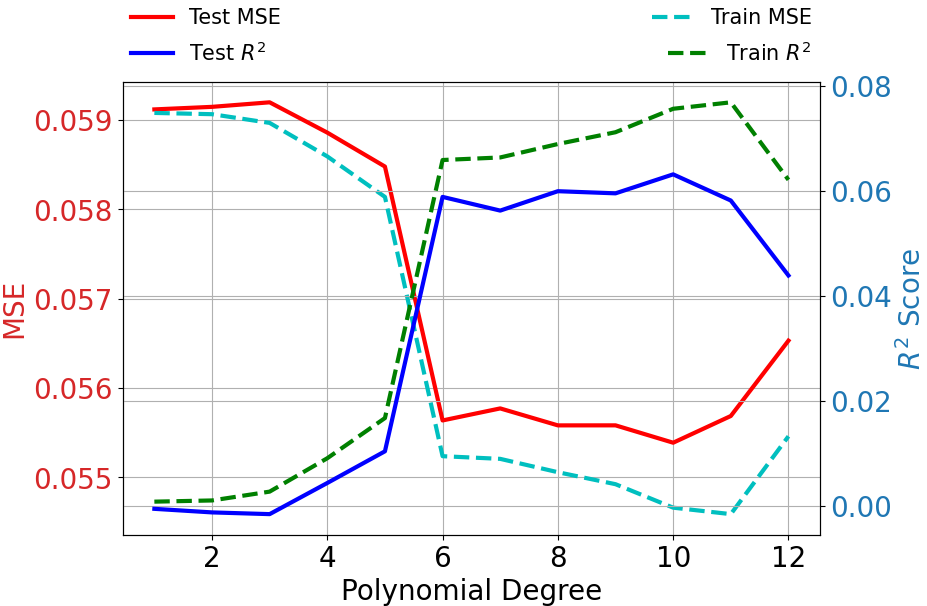
\includegraphics[width=4in,keepaspectratio]{Modelsel_OLS_Terrain}
  \caption{Performance of the OLS regression on the digital terrain data measured by the train and test MSE and $R^2$ sore.}
    \label{Modelsel_OLS_Terrain}
\end{figure}

The fitting and prediction capabilities of the three regression methods are checked by computing the training and testing MSE and $R^2$ scores (see Figure \ref{Modelsel_Ridge_LASSO_scaled_Terrain}). Here, we used the optimal polynomial order as a model and optimal $\lambda$ as a hyper-parameter. The OLS and Ridge regressions have equally the smallest training MSE and $R^2$ score close to $1$. However, all the three regression methods perform poorly on the test data, but the LASSO regression has slightly better MSE and $R^2$ score compared to the other two methods of regression.

Finally, Figure \ref{Confidence_interval_scaled_Terrain} show the coefficients $\mathbf{\beta}$ of the OLS, Ridge, and LASSO regressions when using the optimal model and hyper-parameters. The corresponding $95\%$ confidence interval is also shown for each of the three regression results. Notice, the confidence intervals for all the methods are very small. We believe, this is mainly due to the fact that the three regression methods performed extremely well in the training data.

\begin{figure}[ht]
     \centering
     \begin{subfigure}{.475\textwidth}
         \centering
         \includegraphics[width=1\linewidth]{Modelsel_Ridge_scaled_7_2_Terrain.png}
     \end{subfigure}
     \begin{subfigure}{.475\textwidth}
         \centering
         \includegraphics[width=1\linewidth]{Modelsel_LASSO_scaled_Terrain.png}
     \end{subfigure}
    \caption{Performance of the Ridge (left) and LASSO (right) regressions on the digital terrain data as a function of the hyper-parameter $\lambda$ and the polynomial order and measured by the test MSE.}
    \label{Modelsel_Ridge_LASSO_scaled_Terrain}
\end{figure}

\begin{figure}[H]
  \centering
  \includegraphics[width=\columnwidth]{OLS_Ridge_LASSO_scaled_new_Terrain.png}
  \caption{The fitting (top row) and prediction (bottom row) performance of the OLS, Ridge, and LASSO regressions on the terrain dataset.}
    \label{OLS_Ridge_LASSO_degree8_Terrain}
\end{figure}

\begin{figure}[H]
  \centering
  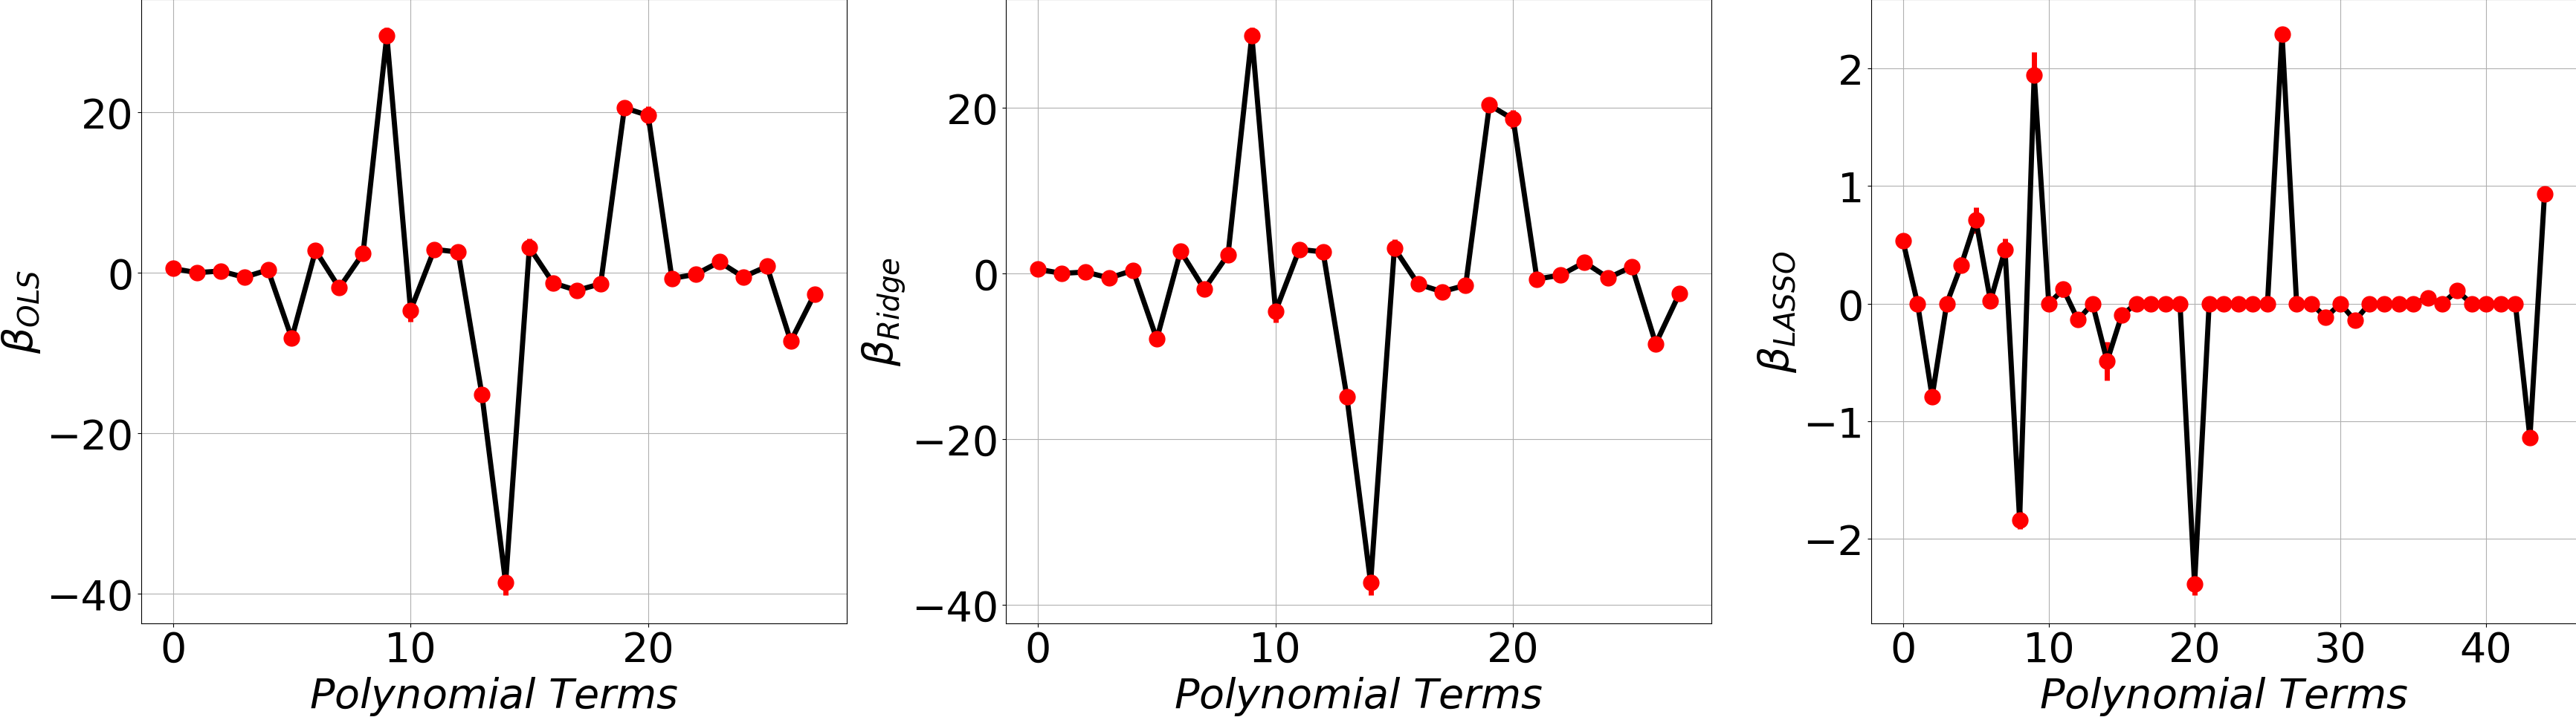
\includegraphics[width=\columnwidth]{Confidence_interval_scaled_Terrain.png}
  \caption{The optimal regression parameters $\mathbf{\beta}$ for the OLS (left), Ridge (middle), and LASSO (right) on the terrain dataset. The $95\%$ confidence interval is also shown. Notice, the polynomial order for the OLS, Ridge, and LASSO are $6$, $6$, and $8$, respectively.}
    \label{Confidence_interval_scaled_Terrain}
\end{figure}

\section{Discussion}
To test the generalizing power of our models, we added noise to our data and introduced testing dataset outside the range of the training. We have found that increasing the number of training data and using simpler models allows us to generalize better than complex models with limited number of data. Moreover, when the size of the training data increases, the in-sample error increases due to the fact that our polynomial models are not powerful enough to learn the true function (i.e., Franke function or the terrain data). However, the out-of-sample error decreases with the size of the training data, because with more data the variance of the model decreases and the training data becomes representative of the distribution from which the Franke function and the terrain data are generated. In the limit of infinite size training data, the in-sample and out-of-sample errors will approach to the same value, which is called the “bias” of our model \cite{Pankaj}.

The bias measures the deviation from the actual value of the function (i.e., Franke function or the terrain data) when we are given an infinite amount of training data. It is also a property of the kind of model we are using to fit the training data. Thus, the more complex the model we use, the smaller the bias. However, the variance, which is a measure of the fluctuation in performance due to finite number of data samples, increases with increasing the complexity of our model. Therefore, the out-of-sample error, which is proportional to the sum of the $Bias^2$ and the variance, will be generally minimized for models with intermediate complexity.

The advantage of shrinkage methods over the OLS is rooted in the bias-variance tradeoff. As $\lambda$ increases, the variance of the model decreases, the bias increases, and the values of the estimator coefficients $\beta$ reduces. Thus, while the OLS suffers from overfitting when the model complexity is large, shrinkage methods regularize the problem by reducing the variance of the model.

The LASSO regression method from \textbf{Scikit-Learn} is computationally demanding when $\lambda < 10^{-4}$. Therefore, in this project we were not able to test the LASSO regression for $\lambda < 10^{-5}$.

For the noisy Franke function data, all the three regression methods performed slightly better on the test data than on the training. However, on the testing terrain dataset all the three regression methods performed poorly. This might be because of the limited size of the training data. It is also possible that polynomial functions are not the best models for predicting terrain data.

\section{Conclusion}
The performance of three regression methods (i.e., OLS, Ridge, and LASSO) is analysed for fitting and predicting using a polynomial function of many orders as a model and a numerically generated, Franke function, and a digital satellite image of a terrain as data sets. Generalization, or getting both the training and the testing errors small is a challenging task for the methods analysed in this project. For the OLS, as the model complexity (i.e., polynomial order) increases, the test error increases while the training error reduces. Using a $5$-fold cross-validation, we found that for the OLS the optimal model is a polynomial order of $7$ on the noisy Franke function and a polynomial order of $6$ on the terrain data. Using models beyond the optimally selected value makes the OLS regression encounter overfitting. To remedy this problem the two shrinkage method (i.e., Ridge and LASSO regressions) are introduced. These methods alleviate overfitting by reducing the variance of the model and consequently increasing the bias. For the noisy Franke function (and terrain) data, the optimal model and hyper-parameter for the Ridge regression are $8^{th}$ ($6^{th}$) order polynomial and $\lambda=10^{-6}$ ($\lambda=10^{-5}$). For the LASSO regression we have $7^{th}$ ($8^{th}$) order polynomial and $\lambda=10^{-5}$ ($\lambda=10^{-5}$). After using the optimal model and the corresponding hyper-parameters, we observed that the Ridge and OLS regressions performed better than the LASSO regression on the noisy Franke function. However, on the terrain dataset, the LASSO regression slightly outperformed both the OLS and Ridge regressions on the prediction of the test data.

%\bibliographystyle{plain}
%\bibliographystyle{siam}
\bibliography{sample}
\bibliographystyle{IEEEtran}
\end{document}
